\documentclass[11pt,a4paper]{article}

\usepackage[T1]{fontenc}
\usepackage{lmodern}
\usepackage{microtype}
\usepackage{graphicx}
\usepackage{xcolor}
\usepackage{geometry}
\usepackage{amsmath}
\usepackage{amssymb}
\usepackage{booktabs}
\usepackage{longtable}
\usepackage{array}
\usepackage{tabularx}
\usepackage{multirow}
\usepackage{float}
\usepackage{caption}
\usepackage{subcaption}
\usepackage{enumitem}
\usepackage{setspace}
\usepackage{fancyhdr}
\usepackage{titlesec}
\usepackage{tcolorbox}
\tcbuselibrary{skins,breakable}
\usepackage{tikz}
\usepackage{siunitx}
\usepackage[numbers,super,sort&compress]{natbib}
\bibliographystyle{unsrtnat}

\geometry{top=2.35cm,bottom=2.35cm,left=2.55cm,right=2.35cm,headheight=22pt}
\definecolor{navy}{HTML}{173F5F}
\definecolor{teal}{HTML}{1B998B}
\definecolor{gold}{HTML}{E9C46A}
\definecolor{orange}{HTML}{E76F51}
\definecolor{red}{HTML}{C94452}
\definecolor{ink}{HTML}{24313D}
\definecolor{soft}{HTML}{F3F6F8}
\definecolor{midgrey}{HTML}{6B7280}

\setstretch{1.12}
\setlength{\parindent}{0pt}
\setlength{\parskip}{0.62em}
\setlength{\emergencystretch}{2em}
\sisetup{detect-all,group-separator={,},group-minimum-digits=4}
\titleformat{\section}{\Large\bfseries\color{navy}}{\thesection}{0.7em}{}
\titleformat{\subsection}{\large\bfseries\color{navy}}{\thesubsection}{0.65em}{}
\titleformat{\subsubsection}{\normalsize\bfseries\color{ink}}{\thesubsubsection}{0.6em}{}
\titlespacing*{\section}{0pt}{1.2em}{0.55em}
\titlespacing*{\subsection}{0pt}{1.0em}{0.4em}
\captionsetup{font=small,labelfont={bf,color=navy},skip=6pt}
\setlist[itemize]{leftmargin=1.5em,itemsep=0.28em,topsep=0.3em}
\setlist[enumerate]{leftmargin=1.6em,itemsep=0.28em,topsep=0.3em}
\newcolumntype{Y}{>{\raggedright\arraybackslash}X}
\newcolumntype{L}[1]{>{\raggedright\arraybackslash}p{#1}}
\newcolumntype{C}[1]{>{\centering\arraybackslash}p{#1}}
\newcolumntype{R}[1]{>{\raggedleft\arraybackslash}p{#1}}
\newcommand{\source}[1]{\par\vspace{2pt}\footnotesize\color{midgrey}Source: #1\par}

\tcbset{
  capstonebox/.style={enhanced,breakable,colback=soft,colframe=navy,boxrule=0.7pt,
    arc=1.5mm,left=3mm,right=3mm,top=2.2mm,bottom=2.2mm,before skip=10pt,after skip=10pt},
  findingbox/.style={enhanced,breakable,colback=teal!7,colframe=teal,boxrule=0.7pt,
    arc=1.5mm,left=3mm,right=3mm,top=2.2mm,bottom=2.2mm,before skip=10pt,after skip=10pt},
  cautionbox/.style={enhanced,breakable,colback=orange!7,colframe=orange,boxrule=0.7pt,
    arc=1.5mm,left=3mm,right=3mm,top=2.2mm,bottom=2.2mm,before skip=10pt,after skip=10pt}
}

\pagestyle{fancy}
\fancyhf{}
\fancyhead[L]{\small\color{midgrey}Data Analytics for Horse Racing}
\fancyhead[R]{\small\color{midgrey}Capstone Interim Report}
\fancyfoot[C]{\small\thepage}
\renewcommand{\headrulewidth}{0.4pt}
\renewcommand{\headrule}{\hbox to\headwidth{\color{navy}\leaders\hrule height \headrulewidth\hfill}}

\graphicspath{{../figures/}{figures/}}

\usepackage{xurl}
\usepackage[
    colorlinks=true,
    linkcolor=navy,
    citecolor=darkgray,
    urlcolor=teal,
    bookmarks=true,
    bookmarksnumbered=true,
    unicode=true
]{hyperref}
\hypersetup{
    pdftitle={Data Analytics for Horse Racing: Prediction and WIN-Betting Evaluation},
    pdfauthor={Chan Hui Man},
    pdfsubject={Capstone Project Interim Report},
    pdfkeywords={horse racing, conditional logit, LightGBM, calibration, betting evaluation, Hong Kong}
}

\begin{document}
\hypersetup{pageanchor=false}

\begin{titlepage}
\thispagestyle{empty}
\vspace*{8mm}
{\color{navy}\rule{\textwidth}{2.2pt}}
\vspace{12mm}
\begin{center}
    {\small\scshape\color{midgrey} Year 4 Capstone Project --- Semester 1 Interim Report\par}
    \vspace{9mm}
    {\Huge\bfseries\color{navy} Data Analytics for\\[2mm] Horse Racing\par}
    \vspace{6mm}
    {\Large\color{ink} Race-Probability Prediction and\\WIN-Betting Evaluation in Hong Kong\par}
    \vspace{12mm}
    \begin{tcolorbox}[width=0.86\textwidth,colback=soft,colframe=navy,arc=2mm,boxrule=0.8pt]
    \centering
    \begin{tabular}{ll}
        \textbf{Student:} & Chan Hui Man \\
        \textbf{Student ID:} & 23087426D \\
        \textbf{Supervisor:} & Prof. Cedric Yiu \\
        \textbf{Department:} & AMA \\
        \textbf{Report date:} & 24 November 2026 \\
    \end{tabular}
    \end{tcolorbox}
    \vfill
    {\small\color{midgrey} Semester 1 empirical analysis and the Semester 2 model-upgrade programme\par}
    \vspace{3mm}
    {\small\color{midgrey} Compiled from reproducible \LaTeX{} source\par}
    \vspace{8mm}
    {\color{navy}\rule{0.55\textwidth}{0.8pt}}
\end{center}
\vfill
\end{titlepage}
\hypersetup{pageanchor=true}

\pagenumbering{roman}
\setcounter{page}{1}
\section*{Abstract}
\addcontentsline{toc}{section}{Abstract}
This report marks the end-of-Semester-1 interim stage of a year-long Year 4 capstone. It develops and evaluates a reproducible data-analytics pipeline for Hong Kong horse racing and defines the Semester 2 research programme. The project addresses two connected questions: whether historical race and runner information can estimate calibrated within-race winning probabilities, and whether those probabilities can support a WIN-betting rule after market prices, pool deductions, and out-of-sample uncertainty are considered. Official Hong Kong Jockey Club fixture, local-results, runner, and dividend pages supply five completed seasons from 2021/22 to 2025/26. The collection contains \num{4214} races and \num{51553} result rows. Removing 404 withdrawn-horse records and excluding seven dead heats from the single-winner likelihood produces a modeling sample of \num{4207} races and \num{51068} starters at 440 result meetings. The chronological design uses 2021/22--2023/24 for training, 2024/25 for validation, and 2025/26 as an untouched test season.

Four candidate estimators compare ridge-regularized conditional-logit and LightGBM models, each with a fundamental specification that excludes odds and a combined specification that includes market information. Historical features are aggregated at entity--race level and shifted before runner expansion so that same-race outcomes cannot leak into predictors. Validation-fitted temperature scaling calibrates probabilities. Evaluation combines race log loss, multiclass Brier loss, top-one strike rate, expected calibration error, runner-level ROC AUC, reliability diagrams, and feature importance. Betting simulations use flat HK\$10 stakes, official WIN dividends, meeting-cluster bootstrap intervals, drawdown, odds-band analysis, and threshold sensitivity grids.

The interim findings show a strong market benchmark and no robust evidence of a profitable edge. On the test season, normalized and calibrated market probabilities attain a race log loss of 2.03209 and a top-one strike rate of 28.65\%. The validation-selected combined conditional logit attains 2.03177 and 29.35\%, respectively. Its log-loss improvement over the market is only 0.000328, with a paired meeting-bootstrap 95\% interval of $[-0.00887,0.00829]$. The prespecified combined-logit value rule places 127 bets and earns HK\$91 on HK\$1,270 staked, an ROI of 7.17\%, but its 95\% interval is $[-49.56\%,77.19\%]$. Returns change materially across thresholds, and every-runner, favourite, top-pick, and fundamental-model strategies lose money. The results therefore support continued methodological development rather than a claim of market-beating performance.

The Semester 2 programme will use rolling-origin evaluation, market-anchored shrinkage, a small feature ablation, calibration-uncertainty diagnostics, and timestamped price scenarios. Any revised model or betting rule will be frozen chronologically and assessed on genuinely new data before a confirmatory claim is made.

{\footnotesize\emph{Research-use notice: this report is an academic analysis of uncertain historical outcomes, not financial or betting advice. Historical returns do not establish future profitability.}}

\clearpage

\tableofcontents
\clearpage
\begingroup
\small
\setstretch{0.92}
\listoffigures
\listoftables
\endgroup
\clearpage

\pagenumbering{arabic}
\setcounter{page}{1}
\section{Research Problem and Project Direction}\label{sec:introduction}

\subsection{Background and rationale}\label{sec:background}
Horse racing is a useful capstone setting for mathematics and data science because each race is a discrete-choice problem with a fixed field, exactly one winner in ordinary circumstances, public covariates, and a market price for every possible outcome. A useful model must therefore do more than label individual runners as likely or unlikely winners. It must compare competitors within the same race, allocate one unit of probability across the field, and quantify uncertainty out of sample. This structure connects multinomial discrete-choice modeling, statistical learning, probability calibration, and decision analysis. Early racetrack research established conditional or multinomial logit models as a natural way to represent within-race competition, while later work demonstrated the practical importance of combining fundamental handicapping variables with public market information\cite{bolton1986,benter1994}.

Hong Kong adds a second layer of analytical interest. Local WIN betting operates through a pari-mutuel pool rather than a fixed-price bookmaker, so final odds summarize public wagering and dividends depend on pool rules. The Hong Kong Jockey Club (HKJC) states that 82.5\% of local WIN pools is paid as dividends, before effects such as rounding and applicable rebates\cite{hkjcguide}. Consequently, an accurate probability forecast need not imply a profitable bet: the price must compensate for both forecast error and the pool deduction. This distinction motivates a project in which predictive quality and economic evaluation are related but separately measured. It also prevents a common analytical mistake in which high winner-selection accuracy is presented as evidence of betting value.

The present report is positioned at the end of Semester 1: data collection, leakage-safe feature construction, baseline modeling, calibration, and the first chronological prediction and WIN-betting evaluation are complete. Semester 2 will be a focused upgrade and confirmation stage. Its priorities are temporal robustness, market-anchored model comparison, better historical information, calibration uncertainty, and realistic betting execution. Section~\ref{sec:plan} specifies the corresponding methods, decision criteria, timeline, and presentation preparation; none of those planned upgrades is presented as an already obtained result.

\subsection{Aim and research questions}\label{sec:aim}
The project aim is to build a transparent, leakage-resistant analytical workflow that estimates within-race winning probabilities for Hong Kong horse races and evaluates whether those estimates improve prediction or historical WIN-betting decisions under a strictly chronological design. The market is treated as a serious benchmark rather than as an inconvenience to be ignored. Fundamental models use only variables available before the outcome and exclude odds; combined models add final market information. This comparison measures the incremental value of the constructed features while retaining a realistic reference point. The design follows the broad logic of fundamental and combined handicapping systems but implements a new, reproducible pipeline on recent official Hong Kong data\cite{benter1994,chapman1994}.

Four research questions organize the interim analysis and the remaining project. They deliberately separate statistical discrimination, calibration, incremental information, and economic value. A model could answer one question favourably and another unfavourably; for example, a top-pick rule could select more winners than a favourite rule while still producing a worse return because of the prices paid. Table~\ref{tab:researchquestions} also identifies the empirical evidence used for each question so that the final report can retain a clear audit trail from aims to conclusions.

\begin{table}[htbp]
\centering
\caption{Research questions and corresponding evidence}\label{tab:researchquestions}
\small
\begin{tabularx}{\textwidth}{L{0.8cm} L{5.3cm} Y L{3.2cm}}
\toprule
\textbf{ID} & \textbf{Research question} & \textbf{Evidence and evaluation} & \textbf{Interim status} \\
\midrule
RQ1 & How well can historical runner, jockey, trainer, and race variables predict the winner without using odds? & Conditional logit and LightGBM compared with uniform and market benchmarks using chronological log loss, Brier loss, top-one strike rate, and ROC AUC. & Answered provisionally using the held-out 2025/26 season. \\
\addlinespace
RQ2 & Are the resulting probabilities numerically calibrated within races? & Race-wise normalization, validation-fitted temperature scaling, reliability diagrams, and expected calibration error. & Answered provisionally; residual bin-level deviations remain. \\
\addlinespace
RQ3 & Does adding market information improve over fundamental-only models, and does it improve over the market itself? & Paired fundamental/combined specifications and paired meeting-bootstrap intervals for differences against the calibrated market. & Market information is essential; incremental improvement over the market is inconclusive. \\
\addlinespace
RQ4 & Can a prespecified expected-value rule generate robust flat-stake WIN returns after pool effects? & Official-dividend settlement, ROI and drawdown, meeting-cluster intervals, odds bands, alternative strategies, and threshold sensitivity. & No robust evidence of profitability in the interim test. \\
\bottomrule
\end{tabularx}
\end{table}

\subsection{Objectives, scope, and unit of analysis}\label{sec:scope}
The first objective is computational: collect official fixtures, race metadata, runner records, final WIN odds, and dividends for five complete seasons and construct a consistent race--runner panel. The second is statistical: develop historical features that use only prior races, estimate race-normalized probabilities, tune on a later validation season, and assess on a subsequent untouched season. The third is evaluative: compare models with proper scoring rules and calibration diagnostics rather than classification accuracy alone. The fourth is decision-oriented: translate probabilities into prespecified betting decisions, settle winning tickets from official dividends, and represent financial uncertainty through clustered resampling and sensitivity analysis. These objectives make the project both mathematically substantive and reproducible.

The unit of prediction is a runner nested within a race, while the unit of model likelihood is the race. The primary betting unit is one HK\$10 WIN stake on at most one selection per race. The study covers Sha Tin and Happy Valley local races in the seasons 2021/22 through 2025/26; the incomplete 2026/27 season is excluded. Only single-winner races enter the present conditional-softmax likelihood, so seven dead heats are removed after data validation. Place pools, exotic bets, Kelly staking, in-play trading, and international simulcasts lie outside the current scope. These boundaries keep the interim analysis tractable and avoid mixing incompatible outcome or settlement mechanisms.

\begin{tcolorbox}[capstonebox]
\textbf{Scope safeguard.} Final WIN odds are used as a proxy for information visible near the start of a race. The analysis is therefore a closing-price backtest, not proof that every simulated trade could have been executed at the stated price. Odds movement after a wager, market impact, rejected bets, and operational delays are not observed in the current dataset. This limitation is central when interpreting the betting results in Section~\ref{sec:results}.
\end{tcolorbox}

\subsection{Interim contribution and report organization}\label{sec:contribution}
The main interim contribution is an end-to-end empirical base rather than a proposal supported only by illustrative examples. The official-source collector has returned all available archived race pages without request errors; the cleaning rules distinguish withdrawn horses from starters; the sample splits are chronological; historical entity features are shifted before being joined back to runners; and every final probability vector has been checked to sum to one within its race. The modeling output includes validation and test metrics, reliability bins, test predictions, feature importance, complete bet records, threshold sensitivity, cumulative profit, and paired uncertainty intervals. These artifacts make the stated findings inspectable and provide a stable foundation for the final-stage extensions.

The remainder of the report follows the analytical sequence. Section~\ref{sec:literature} reviews probability modeling, market efficiency, calibration, and betting evaluation. Section~\ref{sec:data} explains data provenance, cleaning, and descriptive patterns. Section~\ref{sec:methods} specifies features, estimators, calibration, metrics, betting rules, and reproducibility controls. Section~\ref{sec:results} presents interim results without interpreting exploratory thresholds as confirmatory evidence. Sections~\ref{sec:discussion} and~\ref{sec:plan} then discuss validity, limitations, the Semester 2 upgrade programme, and presentation preparation. Appendices contain detailed numerical tables and a reproduction guide.

\section{Literature Review and Conceptual Framework}\label{sec:literature}

\subsection{Race outcomes as discrete choices}\label{sec:lit-logit}
The conditional-logit framework treats each race as a choice set in which one runner is observed to win. Runner covariates enter a latent score, and exponentiating and normalizing those scores within the field produces probabilities that sum to one. This is closely related to McFadden's conditional-logit formulation for qualitative choice and was applied directly to racetrack handicapping by Bolton and Chapman\cite{mcfadden1974,bolton1986}. The key advantage is not merely computational convenience. Race-level normalization encodes the fact that strengthening one competitor necessarily reduces the probability available to the others, whereas independent binary classifiers can produce incoherent race probabilities unless they are post-processed.

Harville's model provides a related route from winning probabilities to ordered finishes through successive without-replacement selection, while Henery and subsequent ranking research consider alternative probability structures for permutations\cite{harville1973,henery1981}. These models matter for a capstone because they clarify what a WIN model does and does not estimate. The present project estimates the first-stage winner probability only; it does not claim that a Harville construction automatically gives accurate place or exacta probabilities. Extending to ordered outcomes would require additional validation because assumptions that are reasonable for a winner market may be inappropriate for lower finishing positions.

A second strand uses flexible statistical learning to capture nonlinear relationships. Benter describes a fundamental handicapping model whose probability estimate is subsequently combined with the public estimate, emphasizing both the difficulty of rivaling public information and the need for out-of-sample assessment\cite{benter1994}. LightGBM is a gradient-boosted tree implementation based on decision-tree ensembles and histogram-oriented learning, making it suitable for nonlinear interactions in tabular data\cite{ke2017lightgbm}. Nevertheless, a conventional binary tree objective does not understand the race choice set. In this project, tree outputs are normalized within each race and compared with a conditional-logit estimator trained directly on race likelihood, allowing the empirical value of flexible learning to be assessed without hiding the structural distinction.

\subsection{Market information and racetrack efficiency}\label{sec:lit-market}
Final odds aggregate information dispersed among bettors, including information absent from a researcher's feature set. In a pari-mutuel WIN pool, prices are linked to the distribution of stakes and the pool deduction rather than being fixed independently by a bookmaker. Bolton and Chapman explicitly connect public probabilities, track take, and expected-return decisions, while Benter reports that a fundamental model must be highly sophisticated to compete with the public estimate\cite{bolton1986,benter1994}. This literature supports two benchmarks in the present study: normalized market probability for prediction and favourite/every-runner rules for economic comparison. A new model is useful only if its performance can be interpreted relative to these simple but demanding references.

The favourite--longshot literature further shows why observed returns should be examined across the odds distribution rather than summarized by a single average. Snowberg and Wolfers document systematically different returns by odds in North American data and evaluate risk-preference and misperception explanations\cite{snowbergwolfers2010}. However, findings from Western markets should not simply be transferred to Hong Kong. Jeong, Kim, and Ro review contrary or reverse-bias evidence in some Asian markets before presenting a different test on Korean racing\cite{jeong2019}. Earlier Hong Kong analysis also motivates market-specific empirical work\cite{chapman1994}. Accordingly, this report treats odds-band returns and calibration as measurements, not as an assumed favourite--longshot pattern.

Market efficiency is not a binary property that one backtest can prove or disprove. A model might approximate final probabilities closely but fail to identify prices with positive expected value; conversely, a small betting profit could arise from luck even when average probability quality is no better than the market. The chance of selecting a threshold after seeing attractive test results adds another concern. The present design therefore distinguishes a prespecified primary betting rule from exploratory threshold grids, reports the number of bets behind every return, and uses paired resampling for both predictive differences and ROI. This interpretation is more conservative than treating a positive historical balance as sufficient evidence of inefficiency.

\subsection{Proper scoring and probability calibration}\label{sec:lit-calibration}
Proper scoring rules provide a principled basis for comparing probabilistic forecasts. Gneiting and Raftery explain that such scores incentivize honest probability statements and summarize their calibration and sharpness properties\cite{gneiting2007}. Race log loss penalizes the negative log probability assigned to the observed winner, while multiclass Brier loss measures squared probability error over the entire field. Both are more informative for this project than winner-selection accuracy alone. A model that selects the same top runner can still receive a very different log loss if it assigns excessive confidence to incorrect outcomes or insufficient probability to the actual winner.

Calibration concerns agreement between stated probabilities and observed frequencies. Niculescu-Mizil and Caruana show that probability estimates from supervised learners can require post-processing and that the best calibration approach depends on the learning method and data regime\cite{niculescu2005}. Temperature scaling offers a deliberately simple one-parameter adjustment: raising probabilities to $1/T$ and renormalizing sharpens or softens the distribution while preserving within-race ranks. It cannot repair every form of local miscalibration, but its low complexity is appropriate for a single validation season. The interim analysis consequently evaluates reliability diagrams and expected calibration error alongside global scores rather than assuming that race-wise normalization alone produces calibrated forecasts.

There is also a conceptual difference between calibration and profitability. A well-calibrated model applied to every runner in a race should tend to reproduce the economics embedded in market prices, including the deduction. Betting only when model expected value exceeds a threshold introduces selection, so small calibration errors can be amplified in the selected subset. This is especially important at long odds, where a one- or two-win difference can change ROI dramatically. Reliability evidence is therefore necessary for interpreting betting output but is not sufficient; settlement, sample size, and selection uncertainty must be reported directly.

\subsection{Validation, betting decisions, and uncertainty}\label{sec:lit-validation}
Randomly dividing runner rows would allow later races and closely related entities to appear on both sides of a split, overstating generalization to a future season. Chronological evaluation instead trains on earlier observations and validates or tests on later ones, consistent with the principle underlying time-ordered cross-validation\cite{sklearn_timesplit}. The present project uses three complete training seasons, one validation season, and one final test season. Hyperparameters and temperature parameters are restricted to training and validation information. Historical features continue to accumulate across split boundaries, but only from races that would already have occurred at prediction time.

The expected-value rule follows directly from probability and decimal odds: a bet is attractive when estimated probability multiplied by gross return exceeds the stake by a sufficient margin. Yet betting evaluation introduces dependence and skew that are easy to underestimate. Races on the same meeting share weather, track condition, and market environment; long-priced selections produce infrequent large returns; and threshold searches create researcher degrees of freedom. The interim analysis therefore clusters bootstrap resampling by meeting, records maximum drawdown, and presents sensitivity as a diagnostic rather than selecting the most profitable cell. This statistical caution reflects the broader warning in racetrack literature that apparent profitability must survive genuine hold-out evaluation\cite{bolton1986,benter1994}.

Table~\ref{tab:lit-synthesis} summarizes how the literature informs specific design choices. It also identifies what the current project adds: a recent five-season Hong Kong panel, explicit same-race leakage controls, race-level and tree-based comparisons under one protocol, official-dividend settlement, and paired uncertainty estimates for both prediction and betting. The contribution is an integrated and auditable empirical workflow, not a claim to have invented conditional logit, boosted trees, calibration, or expected-value wagering.

\begin{table}[htbp]
\centering
\caption{Literature synthesis and implications for this project}\label{tab:lit-synthesis}
\small
\begin{tabularx}{\textwidth}{L{3.5cm} L{4.4cm} Y}
\toprule
\textbf{Research strand} & \textbf{Representative sources} & \textbf{Design implication} \\
\midrule
Discrete-choice and ranking models & McFadden; Harville; Bolton and Chapman; Henery\cite{mcfadden1974,harville1973,bolton1986,henery1981} & Estimate probabilities within a race and reserve ordered-finish models for a separately validated extension. \\
\addlinespace
Fundamental and combined handicapping & Benter; Chapman\cite{benter1994,chapman1994} & Measure incremental information by comparing fundamental and market-augmented specifications out of sample. \\
\addlinespace
Nonlinear tabular learning & Ke et al.\cite{ke2017lightgbm} & Include LightGBM as a flexible comparator, but normalize runner outputs before race evaluation. \\
\addlinespace
Market efficiency and odds patterns & Snowberg and Wolfers; Jeong et al.\cite{snowbergwolfers2010,jeong2019} & Test Hong Kong odds-band behaviour empirically and avoid assuming a Western favourite--longshot pattern. \\
\addlinespace
Scoring and calibration & Gneiting and Raftery; Niculescu-Mizil and Caruana\cite{gneiting2007,niculescu2005} & Use log loss, Brier loss, reliability, and validation-only temperature scaling rather than accuracy alone. \\
\addlinespace
Chronological generalization & Time-series validation documentation\cite{sklearn_timesplit} & Preserve time order in splitting and construct every historical predictor from prior races only. \\
\bottomrule
\end{tabularx}
\end{table}

\section{Data Sources and Sample Construction}\label{sec:data}

\subsection{Official provenance and collection}\label{sec:data-source}
The analysis uses HKJC fixture pages to identify local meetings and HKJC local-results pages to obtain race metadata, runner performance, WIN odds, and dividend tables\cite{hkjcfixtures,hkjcresults}. Collection covers September--July seasons beginning in 2021 and ending in 2026. The fixture parser records date, racecourse, season, and the scheduled number of races. The results parser extracts class and distance text, rating band, going, course configuration, purse, placing, horse number and identifier, jockey, trainer, carried weight, declared body weight, draw, running position, finish time, and displayed WIN odds. The exact WIN dividend per HK\$10 is joined to the winning horse from the official dividend table rather than inferred solely from rounded displayed odds.

The collection was executed on 19 November 2026 with retry logic, local compressed-page caching, and a manifest of request outcomes. There are 444 scheduled meeting--course records, \num{4248} scheduled races on those fixture pages, and \num{4214} archived result races. The difference of 34 races occurs at eight meetings for which the archive contains no result for some or all scheduled races; four of those meetings have no collected result race. This is a coverage difference, not a hidden modeling exclusion. The collector recorded zero request errors across \num{4703} candidate race URLs, including harmless requests beyond the final race number at a meeting. All numerical analysis is based on races for which an official result page was actually retrieved.

\subsection{Cleaning and quality assurance}\label{sec:data-cleaning}
The raw panel contains \num{51553} result rows. Of these, 404 carry HKJC withdrawal codes (WV, WV-A, WX, WX-A, or WXNR) and lack both draw and final WIN odds. An initial audit showed that treating these rows as starters would unnecessarily exclude 383 otherwise valid races and distort field sizes and market probabilities. They are therefore removed before any feature construction. The remaining \num{51149} rows are starters. Seven dead heats are excluded from the present likelihood and its direct evaluation because that likelihood assumes exactly one winner per race; these seven races contain 81 starters, leaving the final \num{4207}-race, \num{51068}-runner modeling sample. Their observed results remain available when subsequent historical features are constructed, because those outcomes would legitimately have been known before later races. No additional race is removed for incomplete odds, draw, carried weight, distance, or winner dividend after this processing.

Quality assurance includes structural and numerical checks. Each included race has exactly one winner, between four and 14 starters, complete market prices, a positive official winner dividend, and the core variables needed by the models. Numeric placings are extracted from labels such as ``1 DH'' before dead heats are identified; non-finishing codes remain non-numeric and receive the worst finishing percentile for historical-form calculations. Probability checks after calibration find a maximum absolute race-sum error below $1.2\times10^{-15}$ across validation and test models. Spot checks against cached official pages also confirmed horse numbers, displayed odds, and exact dividends, including cases where the official dividend differs from ten times the rounded displayed odds.

\begin{table}[htbp]
\centering
\caption{Sample-flow audit from fixture schedule to modeling panel}\label{tab:sampleflow}
\small
\begin{tabularx}{\textwidth}{L{7.3cm} R{2.2cm} Y}
\toprule
\textbf{Stage} & \textbf{Count} & \textbf{Interpretation} \\
\midrule
Scheduled meeting--course records & 444 & HKJC fixture records in five seasons. \\
Scheduled races on fixture pages & \num{4248} & Planned race count before archive availability checks. \\
Archived result races collected & \num{4214} & Official races with a parseable result table. \\
Raw runner result rows & \num{51553} & Includes horses subsequently recorded as withdrawn. \\
Withdrawn rows removed & 404 & Non-starters across 383 races; removed before field-size calculation. \\
Starters after withdrawal removal & \num{51149} & Runners eligible for sample inclusion. \\
Dead-heat races excluded & 7 & Single-winner likelihood restriction; 81 starters removed. \\
Final modeling races / starters & \num{4207} / \num{51068} & Complete cases used for chronological analysis. \\
Result meetings represented & 440 & 88 result meetings in each season. \\
\bottomrule
\end{tabularx}
\source{Project collection manifest, coverage table, and sample-exclusion audit.}
\end{table}

\subsection{Chronological partitioning}\label{sec:data-split}
The seasons are partitioned by time rather than randomly sampled. Seasons 2021/22--2023/24 provide \num{2498} training races and \num{29967} runners; 2024/25 provides 847 validation races and \num{10341} runners; and 2025/26 provides 862 test races and \num{10760} runners. Model regularization, the primary trained model, and calibration temperature are selected or fitted using training and validation information only. The test season is evaluated after those decisions. Historical feature accumulation does not reset at season boundaries, because prior-season information would legitimately be available for a future race, but no current or future outcome enters a predictor.

This design sacrifices the simplicity of random cross-validation in exchange for a more realistic forecasting question. Horse, jockey, and trainer populations evolve; class compositions and market behaviour can drift; and the same entities naturally recur across training and test periods. Such recurrence is not itself leakage because only earlier outcomes are used. The principal remaining threat is temporal distribution shift, which cannot be eliminated by splitting. It is assessed indirectly by comparing validation and test metrics and will be examined more fully through rolling-origin experiments in the remaining work.

\begin{table}[htbp]
\centering
\caption{Chronological data partition}\label{tab:split}
\small
\begin{tabular}{L{4.1cm} L{3.2cm} R{2.0cm} R{2.2cm} C{2.3cm}}
\toprule
\textbf{Season(s)} & \textbf{Role} & \textbf{Races} & \textbf{Runners} & \textbf{Result meetings} \\
\midrule
2021/22--2023/24 & Training & \num{2498} & \num{29967} & 264 \\
2024/25 & Validation and calibration & 847 & \num{10341} & 88 \\
2025/26 & Untouched test & 862 & \num{10760} & 88 \\
\midrule
\textbf{Total} & & \textbf{\num{4207}} & \textbf{\num{51068}} & \textbf{440} \\
\bottomrule
\end{tabular}
\end{table}

\begin{figure}[htbp]
\centering
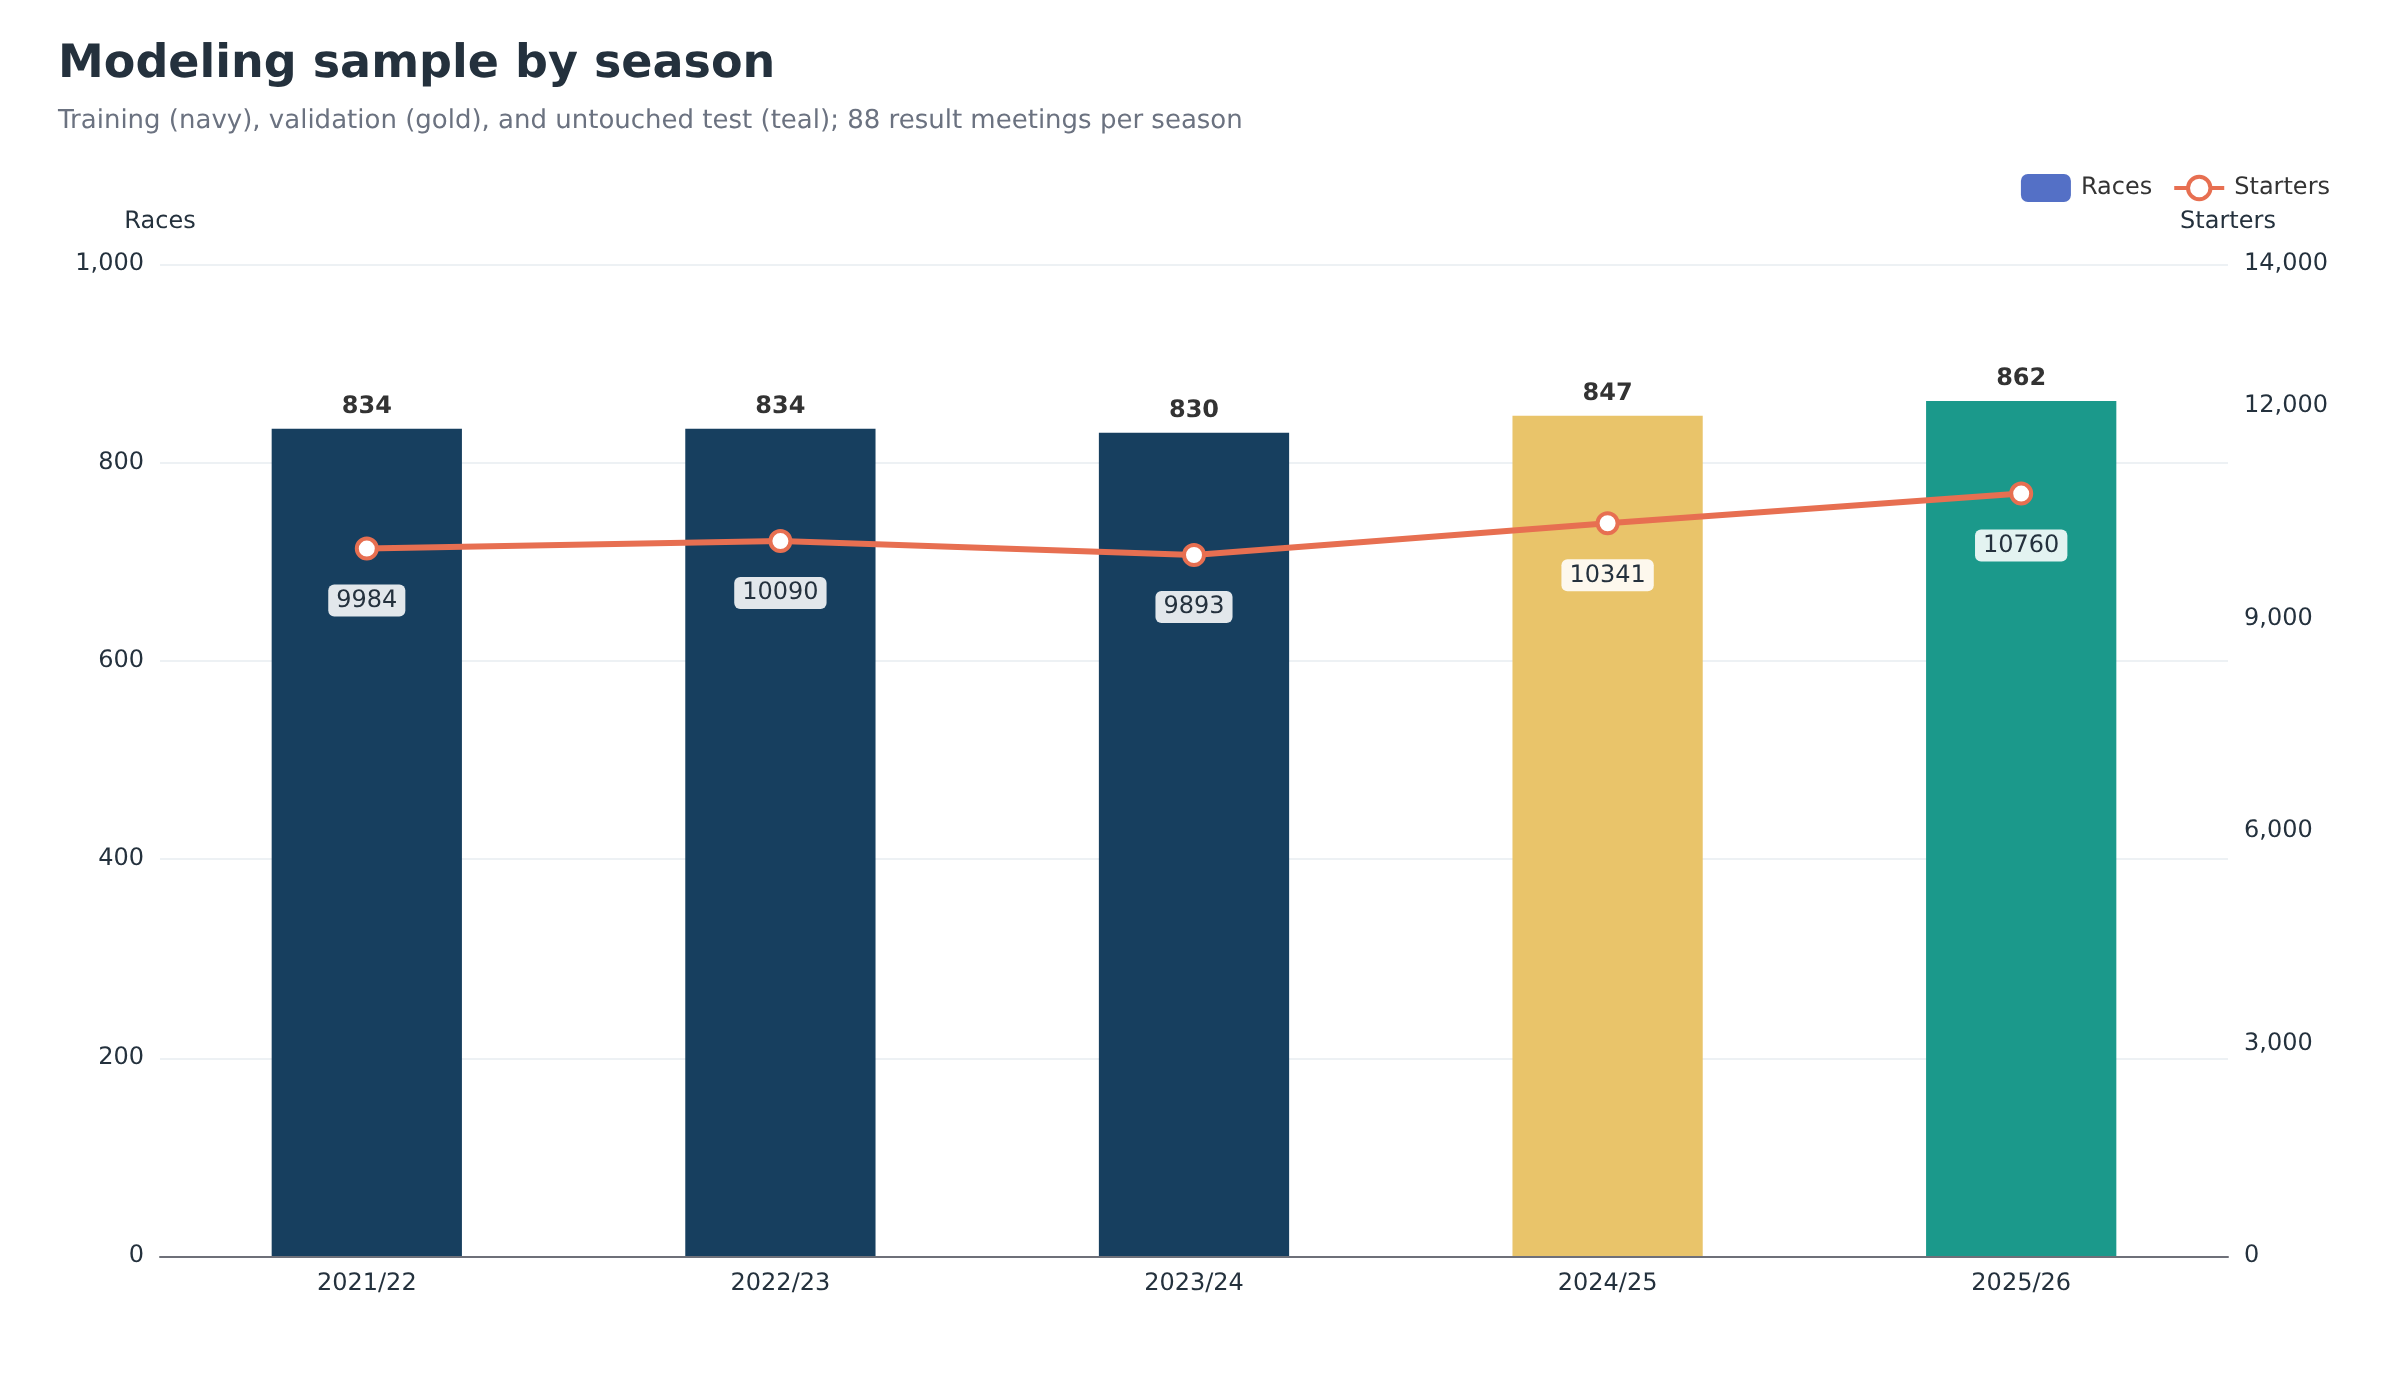
\includegraphics[width=0.96\textwidth]{season_sample.png}
\caption{Season-level modeling sample and chronological roles. Bar labels give races; line labels give starters. The first three seasons form training, 2024/25 is validation, and 2025/26 is the untouched test.}\label{fig:season-sample}
\end{figure}

\subsection{Descriptive characteristics}\label{sec:data-descriptive}
Table~\ref{tab:season-descriptives} shows that the sample is broadly stable in scale but not identical across seasons. Mean field size rises from 11.92 in 2023/24 to 12.48 in the test season, while the average race overround remains close to 1.227--1.228. Here overround is the sum of reciprocal displayed decimal odds within a race, and normalized market probability is each reciprocal divided by that sum. This normalization removes the mechanical scale excess but does not by itself prove calibration or remove dividend rounding. The similarity of overround across seasons makes the chronological comparisons easier to interpret, although it does not rule out changes in other market characteristics.

Observed favourite performance varies across seasons. The single lowest-odds selection, with horse number breaking ties, wins 33.45\% of races in 2022/23 but 28.65\% in 2025/26. These are descriptive frequencies, not by themselves evidence of structural non-stationarity: with roughly 830--860 races per season, sampling uncertainty is material. The variation nevertheless cautions against treating one season's favourite strike rate as a fixed parameter. It also anticipates the distinction between prediction and return: even when favourites win approximately three races in ten, their average price can be insufficient to cover stakes and pool effects. Section~\ref{sec:results-betting} therefore evaluates both outcomes and official-dividend returns.

\begin{table}[htbp]
\centering
\caption{Descriptive statistics by season}\label{tab:season-descriptives}
\small
\begin{tabular}{L{2.1cm} R{1.3cm} R{1.6cm} R{1.6cm} R{1.9cm} R{1.9cm}}
\toprule
\textbf{Season} & \textbf{Races} & \textbf{Mean field} & \textbf{Mean overround} & \textbf{Favourite win rate} & \textbf{Runners} \\
\midrule
2021/22 & 834 & 11.97 & 1.22782 & 28.90\% & \num{9984} \\
2022/23 & 834 & 12.10 & 1.22803 & 33.45\% & \num{10090} \\
2023/24 & 830 & 11.92 & 1.22766 & 29.40\% & \num{9893} \\
2024/25 & 847 & 12.21 & 1.22757 & 32.82\% & \num{10341} \\
2025/26 & 862 & 12.48 & 1.22694 & 28.65\% & \num{10760} \\
\bottomrule
\end{tabular}
\source{Race-level means use one observation per race. Favourite ties are broken by horse number.}
\end{table}

\section{Analytical Methodology}\label{sec:methods}

\subsection{Within-race probability framework}\label{sec:methods-probability}
Let race $r$ contain $n_r$ starters and let $x_{ri}$ denote the feature vector for runner $i$. A model produces a nonnegative raw score $a_{ri}$, which is converted into a probability distribution over the field by
\begin{equation}
p_{ri}=\Pr(Y_r=i\mid x_{r1},\ldots,x_{rn_r})
=\frac{a_{ri}}{\sum_{j=1}^{n_r}a_{rj}},
\qquad \sum_{i=1}^{n_r}p_{ri}=1.
\label{eq:race-probability}
\end{equation}
For the conditional-logit specifications, $a_{ri}=\exp(s_{ri})$ and $s_{ri}=x_{ri}^{\top}\beta$. For LightGBM, $a_{ri}$ is the clipped binary-classifier output followed by the same race-wise normalization. This common output contract allows all models and benchmarks to be evaluated using identical race metrics and betting rules.

Two transparent benchmarks anchor the analysis. The uniform benchmark sets $p_{ri}=1/n_r$. The market benchmark uses displayed decimal WIN odds $d_{ri}$ to compute
\begin{equation}
q_{ri}=\frac{1/d_{ri}}{\sum_{j=1}^{n_r}1/d_{rj}},
\qquad
O_r=\sum_{j=1}^{n_r}\frac{1}{d_{rj}},
\label{eq:market-probability}
\end{equation}
where $O_r$ is the race overround. The quantity $q_{ri}$ is a normalized implied probability, not an assumption that odds reveal the true probability exactly. All non-uniform probability vectors, including the market benchmark, receive the same validation-fitted temperature adjustment described below. Because temperature transformation is monotonic within a race, it changes log loss and calibration but not top-one selections.

\subsection{Predictor engineering and leakage prevention}\label{sec:methods-features}
The fundamental specification contains 36 runner-level variables representing recent form, longer-run performance, connections, race-relative physical conditions, changes from the previous observed start, and draw interactions. Table~\ref{tab:feature-groups} summarizes the groups. LightGBM additionally receives race-level context and categorical variables; these are excluded from conditional logit when they are constant for every runner in a race because such constants cancel from Equation~\eqref{eq:race-probability}. The combined conditional logit adds $\log q_{ri}$. Combined LightGBM adds $\log q_{ri}$, $\log d_{ri}$, market rank, and overround. Thus no fundamental model indirectly receives an odds-derived variable.

Historical predictors are constructed only from prior races. For each horse, distance-specific horse record, course-specific horse record, jockey, and trainer, results are first aggregated to entity--race level. This step is essential when a trainer or jockey has multiple mounts in one race: expanding runner rows before aggregation could allow one runner's current outcome to contaminate another runner's predictor. Cumulative totals are then shifted before being merged back to the race--runner panel. For entity $e$ at chronological race $t$, define prior mounts $N_{et}$ and prior wins $W_{et}$ by sums over races strictly before $t$. A smoothed historical win rate is
\begin{equation}
\widetilde{w}_{et}=\frac{W_{et}+\alpha/12}{N_{et}+\alpha},
\label{eq:smoothed-rate}
\end{equation}
with analogous place and mean-finish estimates centred at 0.25 and 0.5, respectively. The smoothing strengths $(\alpha_{\mathrm{win}},\alpha_{\mathrm{place}},\alpha_{\mathrm{finish}})$ are $(24,24,16)$ for horses, $(12,12,8)$ for distance/course records, $(60,60,40)$ for jockeys, and $(80,80,50)$ for trainers.

\begin{table}[htbp]
\centering
\caption{Feature groups and their intended information}\label{tab:feature-groups}
\small
\begin{tabularx}{\textwidth}{L{3.2cm} Y L{3.8cm}}
\toprule
\textbf{Group} & \textbf{Representative variables} & \textbf{Availability and processing} \\
\midrule
Horse career history & Log prior starts, smoothed win/place rates, mean finishing percentile, days since previous start, first observed-start indicator & Prior races only; first observed start is not asserted to be the horse's true lifetime debut. \\
\addlinespace
Recent form & Last finishing percentile, last-three mean finish, last-three win rate & Shifted before rolling calculations; non-finish codes receive worst percentile. \\
\addlinespace
Context records & Distance- and course-specific starts, win/place rates, and mean finish & Entity--race aggregation and chronological shift; stronger smoothing for sparse records. \\
\addlinespace
Jockey and trainer & Log prior mounts, win/place rates, mean finish & Same-race mounts aggregated before shifting to prevent cross-runner leakage. \\
\addlinespace
Race-relative condition & Carried-weight and body-weight deviations from race mean; normalized draw and squared draw & Current race-card information; no result fields used. \\
\addlinespace
Changes and interactions & Weight, body-weight, distance, and class changes; draw interactions with sprint, Happy Valley, and all-weather racing & Changes use the previous observed start; interactions allow context-specific draw association. \\
\addlinespace
Additional LightGBM context & Field size, distance, class score, course, surface, going, class name, course configuration & Median-imputed numerics and training-fitted one-hot encoding. \\
\addlinespace
Combined-only market inputs & Log normalized market probability; additionally log odds, market rank, and overround for LightGBM & Computed from final odds of all starters; excluded from every fundamental specification. \\
\bottomrule
\end{tabularx}
\end{table}

\subsection{Conditional-logit estimation}\label{sec:methods-logit}
For ordinary races with one observed winner $w_r$, the conditional-logit parameters minimize a race-averaged negative log likelihood with ridge regularization:
\begin{equation}
\widehat{\beta}
=\arg\min_{\beta}\left[
-\frac{1}{R}\sum_{r=1}^{R}
\left(x_{rw_r}^{\top}\beta-\log\sum_{j=1}^{n_r}\exp(x_{rj}^{\top}\beta)\right)
+\frac{\lambda}{2}\lVert\beta\rVert_2^2
\right].
\label{eq:clogit-objective}
\end{equation}
The optimization uses analytically derived gradients and L-BFGS-B. Numerical stability is obtained by subtracting the maximum score within each race before exponentiation. Numeric predictors are median-imputed and standardized using statistics fitted on training data only. Separate fundamental and combined preprocessors ensure that the combined market column does not alter the scaling of fundamental variables.

The ridge penalty is selected from $\{0.0001,0.001,0.01,0.1\}$ by validation race log loss. The selected values are 0.1 for the fundamental specification and 0.01 for the combined specification. Only the validation season informs this choice. The resulting models are then applied to the test season without refitting on validation outcomes, keeping the evaluation straightforward to audit. A future extension can refit on training plus validation after all design decisions are frozen, but the interim results deliberately retain the original train-only fitted models.

\subsection{LightGBM estimation and model selection}\label{sec:methods-lgbm}
The LightGBM comparator uses a binary log-loss objective with 350 trees, learning rate 0.025, 15 leaves, minimum child size 100, feature fraction 0.85, subsample fraction 0.9, L1 regularization 0.2, and L2 regularization 5.0. Runner weights equal $1/n_r$, so each race contributes equal total weight despite varying field sizes. Numeric missing values receive training medians and categorical variables use training-fitted one-hot encoding. Predicted binary scores are clipped to $[10^{-12},1-10^{-12}]$ and normalized within each race before evaluation. This is a pragmatic adaptation, not a claim that the binary booster optimizes conditional race likelihood directly.

The hyperparameters are fixed across fundamental and combined models to limit validation searching and isolate the effect of feature information. Four trained candidates arise: fundamental conditional logit, fundamental LightGBM, combined conditional logit, and combined LightGBM. The \emph{primary trained model} is the candidate with the lowest validation log loss; uniform and market remain benchmarks rather than candidates for this label. Combined conditional logit is selected with validation log loss 2.00168. Importantly, the calibrated market itself performs better on validation log loss (1.98864), so the selection terminology must not be misread as evidence that the trained model dominates the market.

\subsection{Temperature calibration and evaluation metrics}\label{sec:methods-metrics}
Temperature scaling adjusts an existing race probability vector using one positive parameter $T$:
\begin{equation}
p_{ri}(T)=\frac{p_{ri}^{1/T}}{\sum_{j=1}^{n_r}p_{rj}^{1/T}}.
\label{eq:temperature}
\end{equation}
For $T<1$ the distribution becomes sharper; for $T>1$ it becomes softer. The optimal $\log T$ is obtained by bounded one-dimensional minimization of validation winner log loss, with $\log T\in[-1.5,1.5]$, and then applied unchanged to test predictions. Fitted temperatures are 0.91977 for market, 0.93338 for fundamental logit, 0.92458 for fundamental LightGBM, 1.00260 for combined logit, and 0.97968 for combined LightGBM. The near-unit value for combined logit indicates almost no global calibration adjustment.

Let $y_{ri}=\mathbf{1}\{i=w_r\}$. The principal predictive metrics are
\begin{align}
\mathrm{LL}&=-\frac{1}{R}\sum_{r=1}^{R}\log p_{rw_r}, \label{eq:logloss}\\
\mathrm{Brier}&=\frac{1}{R}\sum_{r=1}^{R}\sum_{i=1}^{n_r}(p_{ri}-y_{ri})^2. \label{eq:brier}
\end{align}
Lower values are better for both. Top-one strike rate is the proportion of races in which the maximum-probability runner wins. Runner-level expected calibration error (ECE) uses ten within-model quantile bins and weights $|\bar p_b-\bar y_b|$ by bin count. Reliability diagrams display the same bin means. Runner-level ROC AUC is reported as a secondary discrimination statistic, but it is not a proper race score: unequal field sizes mean even uniform within-race probabilities need not have AUC 0.5. Similarly, uniform ECE can be mechanically zero when bins coincide with field sizes, so neither statistic is interpreted in isolation.

\subsection{WIN-betting rules and exact settlement}\label{sec:methods-betting}
For decimal odds $d_{ri}$, the model-implied expected gross-profit multiple per unit stake is
\begin{equation}
\widehat{EV}_{ri}=p_{ri}d_{ri}-1.
\label{eq:expected-value}
\end{equation}
The prespecified primary value rule considers runners with $\widehat{EV}_{ri}>0.05$ and $d_{ri}\leq30$, then places one HK\$10 stake on the runner with the largest expected value in each qualifying race. If no runner qualifies, no bet is placed. Comparator strategies bet on the maximum-probability runner in every race, the lowest-odds favourite in every race, and every runner in every race. Value strategies are also reported for the other trained models. Horse number breaks favourite ties, and deterministic sorting makes all selections reproducible.

Winning bets are settled using the official HKJC WIN dividend $D_{ri}$ for a HK\$10 unit, not by assuming that rounded odds reproduce the payout exactly. Net profit is $D_{ri}-10$ for a winning selection and $-10$ otherwise. Total ROI is total net profit divided by total stakes. This automatically incorporates the pool economics reflected in official dividends. The HKJC guide states an 82.5\% dividend percentage for local WIN pools and describes conditional rebates for sufficiently large losing tickets\cite{hkjcguide}; no rebate is assumed in the conservative flat-stake analysis. Maximum drawdown is the greatest decline from a previous cumulative-profit peak, including zero as the initial capital reference.

\subsection{Uncertainty and reproducibility controls}\label{sec:methods-uncertainty}
ROI confidence intervals use 3,000 meeting-cluster bootstrap resamples. All bets on one calendar meeting form a cluster; cluster indices are drawn with replacement, and paired profits and stakes are summed before each ROI is calculated. This preserves dependence and varying bet counts within meetings. Predictive comparisons against the market use 5,000 paired meeting-cluster resamples of race-level log-loss, Brier-loss, and top-one differences. Intervals are percentile intervals. They quantify sampling instability under this resampling scheme, not model-selection uncertainty, execution uncertainty, or a guarantee about future seasons.

The random seed is \num{20261119}. Analysis outputs include the cleaned panel, race predictions, model metrics, reliability bins, feature gains, coefficients, complete bet ledgers, cumulative-profit sequences, sensitivity grids, and collection manifests. Every reported probability vector is checked for finiteness and unit race sums. Betting counts and totals can be reconstructed from the saved bet-level files, and every runner row retains its official source URL. These controls provide the reproducibility needed for supervisor review and for extending rather than rebuilding the project during the final stage.

\section{Interim Empirical Results}\label{sec:results}

\subsection{Predictive performance on validation and test seasons}\label{sec:results-prediction}
Table~\ref{tab:model-metrics} reports the complete validation and test comparison after temperature calibration. The uniform benchmark has test log loss 2.51622, while the market attains 2.03209. Fundamental models lie between these references: fundamental logit attains 2.24708 and fundamental LightGBM 2.24613. Their top-one strike rates are 22.85\% and 23.43\%, respectively, compared with 11.95\% for uniform and 28.65\% for market. This answers RQ1 provisionally: historical features contain substantial predictive information, but the constructed fundamental specifications remain well behind final market prices on the untouched season.

Adding market variables closes almost all of that gap. Combined logit has validation log loss 2.00168, the lowest among the four trained candidates, and is therefore the primary trained model. Its test log loss is 2.03177, only 0.000328 below the market value, and its top-one rate is 29.35\%, 0.696 percentage points above the market/favourite rate. Combined LightGBM performs slightly worse at 2.04694. The validation result also warns against overstatement: calibrated market log loss is 1.98864, better than every trained candidate, including combined logit. Thus the main finding is approximate market equivalence on test, not a consistent forecasting advantage.

\begin{table}[htbp]
\centering
\caption{Calibrated probability-model performance}\label{tab:model-metrics}
\small
\setlength{\tabcolsep}{3.5pt}
\begin{tabular}{L{3.8cm} R{1.85cm} R{1.45cm} R{1.5cm} R{1.5cm} R{1.4cm} R{1.4cm}}
\toprule
\textbf{Model} & \textbf{Validation LL} & \textbf{Test LL} & \textbf{Test Brier} & \textbf{Test top-one} & \textbf{Test ECE} & \textbf{Test AUC} \\
\midrule
Uniform & 2.49199 & 2.51622 & 0.91845 & 11.95\% & 0.00000 & 0.53248 \\
Market & \textbf{1.98864} & 2.03209 & \textbf{0.81882} & 28.65\% & 0.00573 & 0.79187 \\
Fundamental logit & 2.20062 & 2.24708 & 0.86938 & 22.85\% & 0.00672 & 0.72515 \\
Fundamental LightGBM & 2.21361 & 2.24613 & 0.86923 & 23.43\% & \textbf{0.00325} & 0.72504 \\
Combined logit & \underline{2.00168} & \textbf{2.03177} & 0.81946 & \textbf{29.35\%} & 0.00574 & \textbf{0.79198} \\
Combined LightGBM & 2.01057 & 2.04694 & 0.82213 & 28.54\% & 0.00663 & 0.78802 \\
\bottomrule
\end{tabular}
\source{Bold test entries indicate the best numerical value; the underlined validation entry identifies the primary trained candidate. Market is a benchmark, not a trained candidate. Lower LL, Brier, and ECE are better; higher top-one and AUC are better.}
\end{table}

\begin{figure}[htbp]
\centering
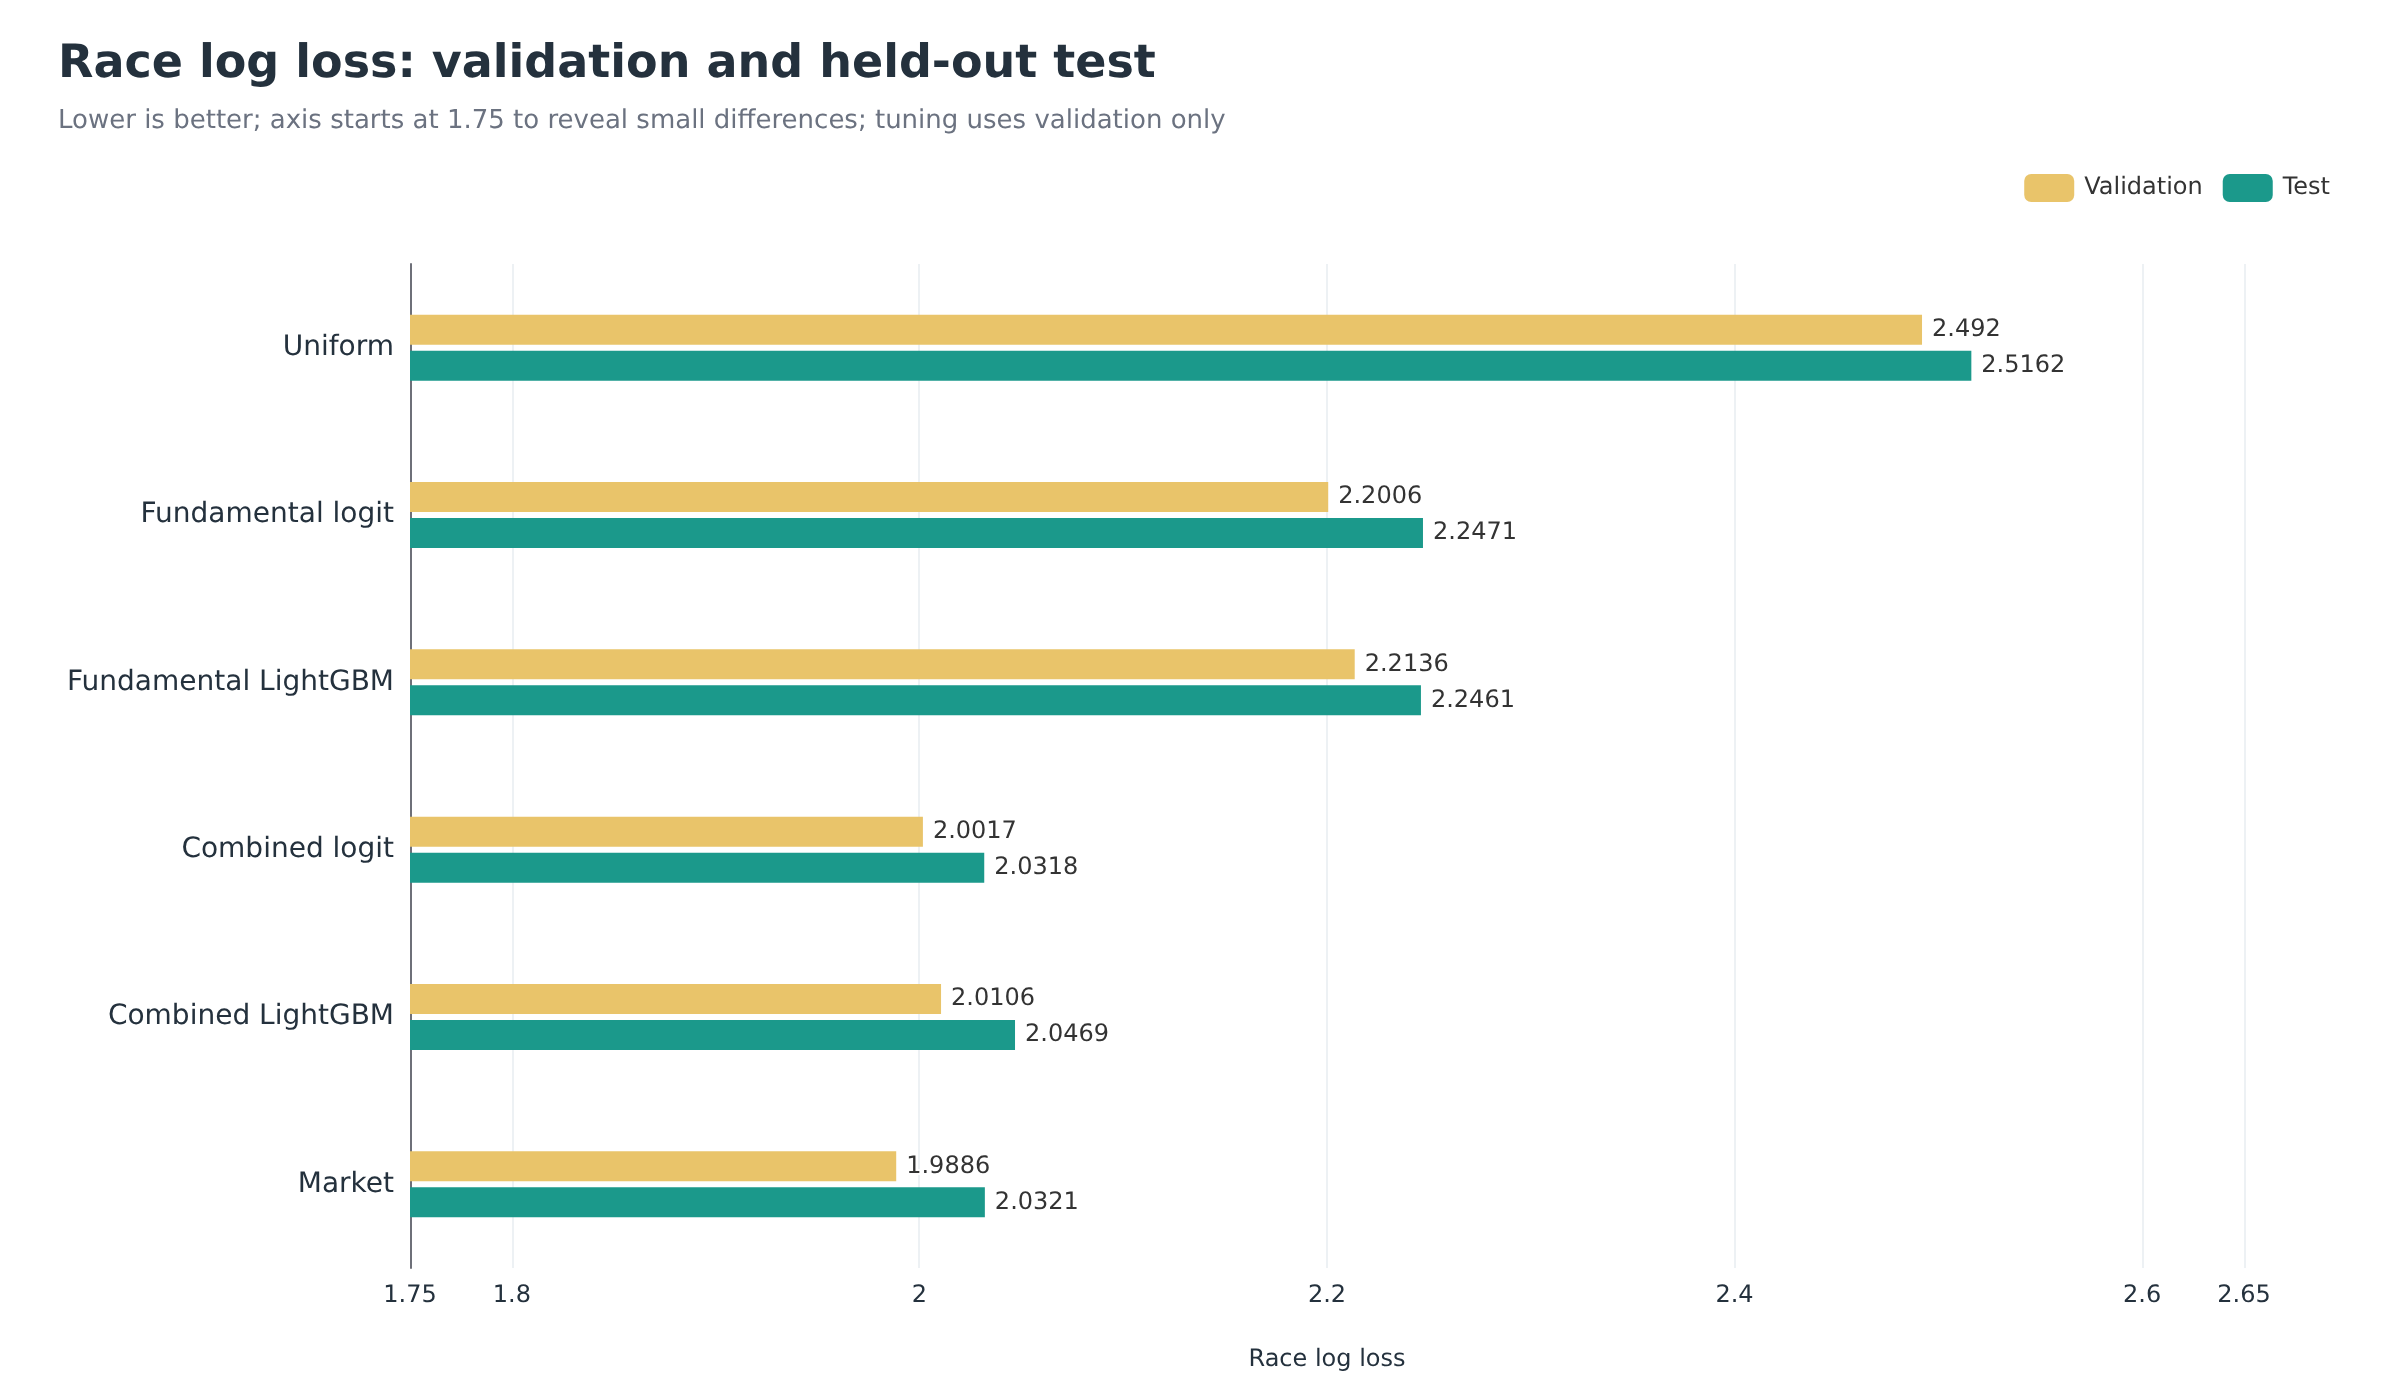
\includegraphics[width=0.97\textwidth]{model_comparison.png}
\caption{Validation and test race log loss. The horizontal axis is truncated to make small differences visible; numerical labels provide the actual scores.}\label{fig:model-comparison}
\end{figure}

Paired meeting-bootstrap intervals reinforce the cautious interpretation. For combined logit minus market, the test log-loss difference is $-0.000328$ with 95\% interval $[-0.008867,0.008288]$. The Brier difference is $+0.000650$ with interval $[-0.002300,0.003498]$, and the top-one difference is $+0.696$ percentage points with interval $[-0.692,2.100]$ points. All three intervals include zero. Combined LightGBM's log-loss difference is $+0.01484$ with interval $[0.00098,0.02900]$, indicating a small disadvantage relative to the market under this resampling analysis. Fundamental-model disadvantages are much larger and their intervals are clearly above zero for log loss.

\begin{table}[htbp]
\centering
\caption{Paired test differences: primary combined logit minus market}\label{tab:paired-differences}
\small
\begin{tabular}{L{3.4cm} R{2.5cm} R{3.5cm} L{3.9cm}}
\toprule
\textbf{Metric} & \textbf{Difference} & \textbf{95\% meeting-bootstrap interval} & \textbf{Interpretation} \\
\midrule
Race log loss & $-0.000328$ & $[-0.008867,\ 0.008288]$ & No resolved difference; negative would favour the model. \\
Multiclass Brier loss & $+0.000650$ & $[-0.002300,\ 0.003498]$ & No resolved difference; positive would favour the market. \\
Top-one strike rate & $+0.696$ pp & $[-0.692,\ 2.100]$ pp & No resolved difference; positive would favour the model. \\
\bottomrule
\end{tabular}
\source{5,000 paired meeting-cluster resamples; pp denotes percentage points.}
\end{table}

\subsection{Calibration and reliability}\label{sec:results-calibration}
Global ECE values are small in absolute terms, ranging from 0.00325 for fundamental LightGBM to 0.00672 for fundamental logit among the non-degenerate models. Figure~\ref{fig:reliability} shows why these summaries should still be accompanied by bin-level inspection. Market, combined-logit, and fundamental-LightGBM probabilities broadly follow the diagonal, but deviations vary across the probability range. In the highest market decile, for example, mean predicted probability is 30.08\% and observed frequency is 28.44\%; in the preceding decile, prediction is 15.70\% and observation 16.73\%. A single global temperature cannot remove all such local differences.

The reliability curves also show that the fundamental model is not uninformative. Its probabilities span a useful range and track observed frequencies approximately, despite weaker log loss and discrimination than the market. This pattern is consistent with information that is genuinely predictive but already largely incorporated into prices. The near-unit combined-logit temperature (1.00260) suggests that its validation likelihood required negligible global sharpening or softening. By contrast, the market temperature of 0.91977 sharpens normalized market probabilities. These are global parameters fitted on one validation season, so their stability across alternative periods remains a final-stage question.

\begin{figure}[htbp]
\centering
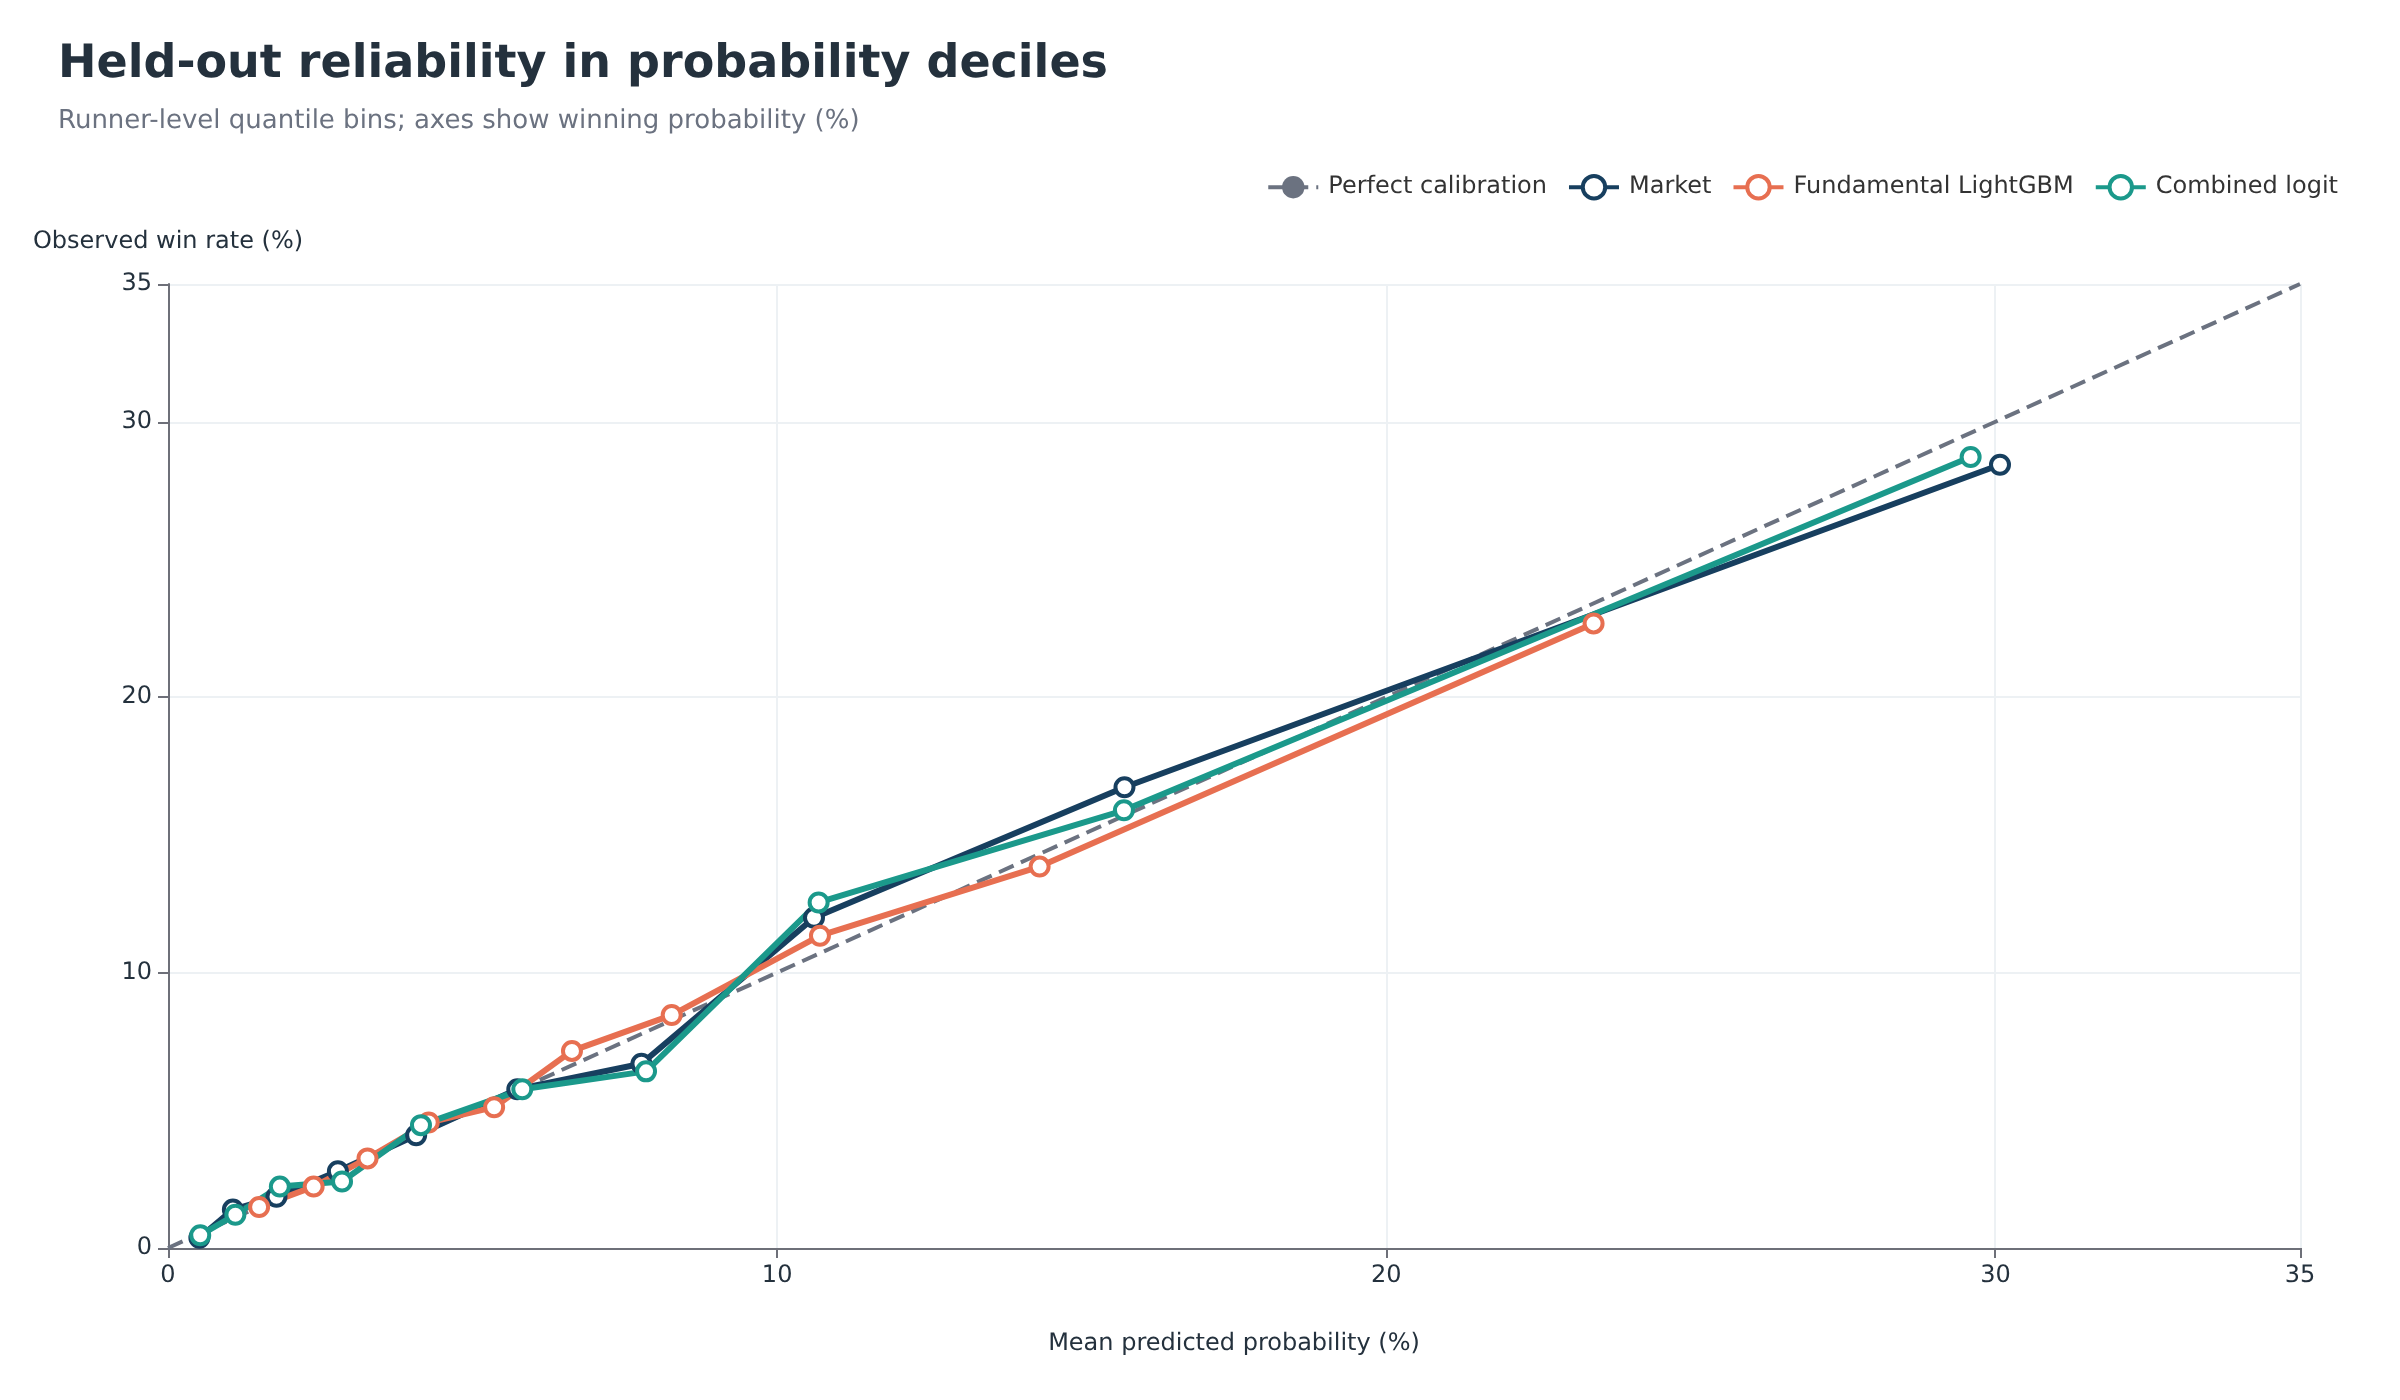
\includegraphics[width=0.96\textwidth]{reliability.png}
\caption{Held-out reliability curves using ten runner-level quantile bins per model. The dashed line denotes perfect calibration.}\label{fig:reliability}
\end{figure}

\subsection{Feature importance and model behaviour}\label{sec:results-importance}
Figure~\ref{fig:importance} displays LightGBM gain importance. In the fundamental model, last-three finishing form contributes 24.27\% of total gain, most recent finish 13.94\%, jockey mean finish 9.64\%, jockey place rate 5.86\%, and normalized draw 3.52\%. The prominence of recent form is consistent with the modeling rationale, but the values are not causal effects. Correlated variables can share or substitute for one another across trees, and gain importance measures use within the fitted ensemble rather than independent information content.

The combined model is dominated by final market variables: log WIN odds contribute 42.32\% and log normalized market probability 36.47\%, together 78.79\% of total gain. Relative carried weight is a distant third at 1.43\%. This concentration explains why adding fundamental variables produces only a small change relative to the market benchmark. It also cautions against interpreting the two market columns separately because they are deterministically related within a race. Future ablation and two-stage residual modeling will be more informative than adding further correlated transformations of the same final price.

\begin{figure}[htbp]
\centering
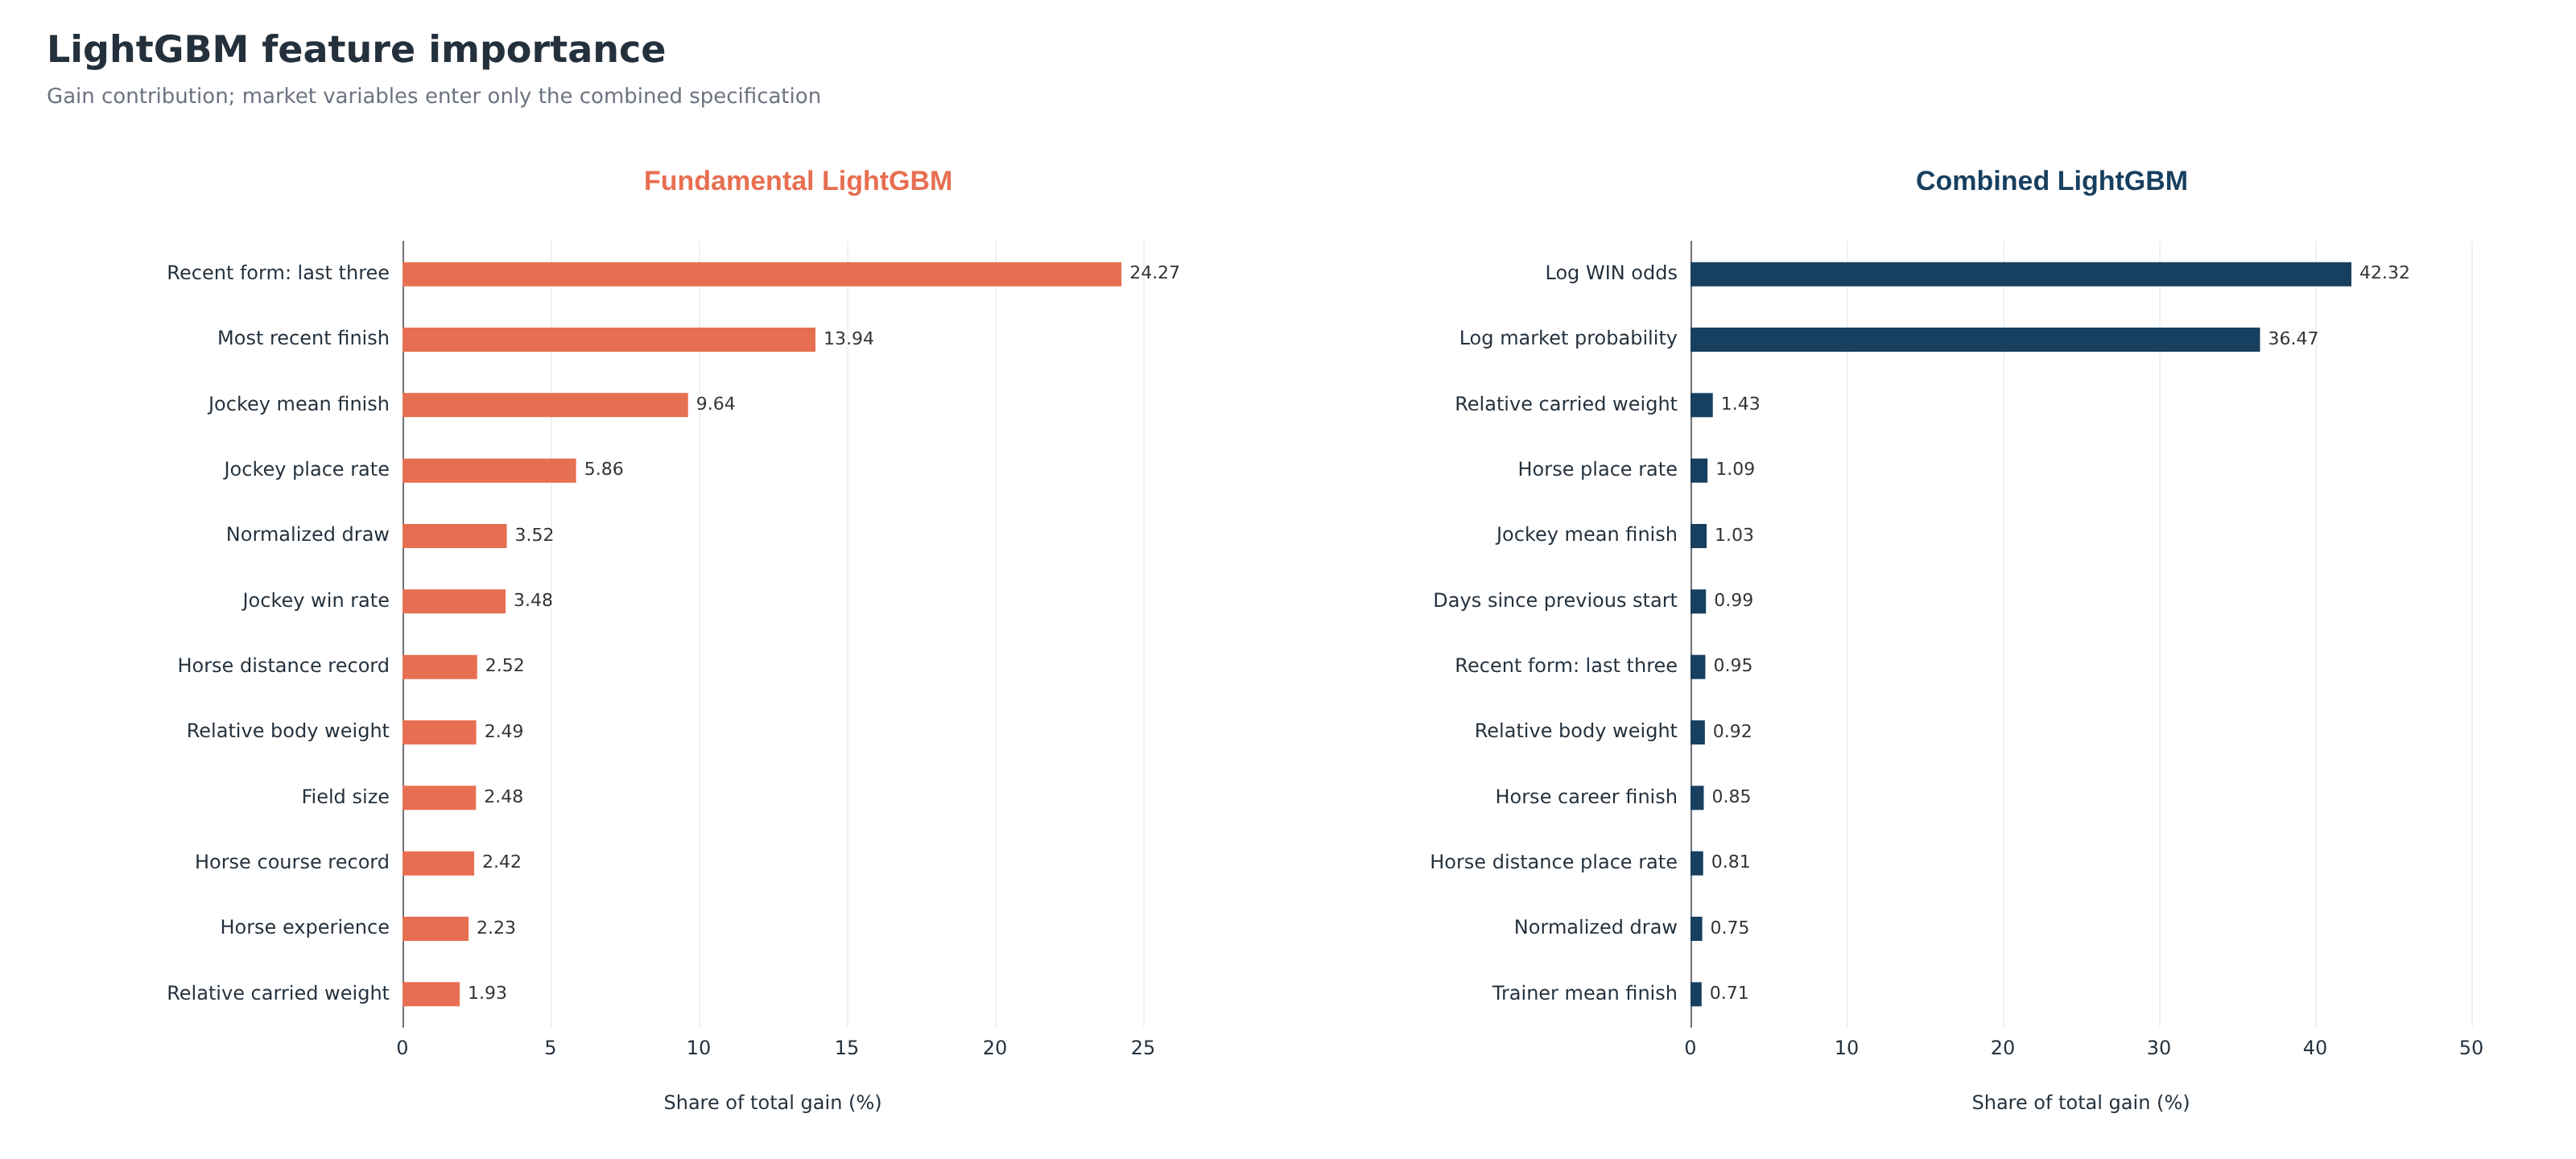
\includegraphics[width=0.99\textwidth]{feature_importance.png}
\caption{LightGBM gain importance for the twelve largest contributors in each specification. Percentages sum over all ensemble features, not only the displayed subset.}\label{fig:importance}
\end{figure}

\subsection{Odds-band calibration and unconditional returns}\label{sec:results-odds}
Before examining model-selected bets, it is useful to ask whether simple price bands already show strong market patterns. Figure~\ref{fig:odds-bands} compares mean normalized market probability with observed win frequency and reports ROI from betting HK\$10 on every runner in each test-season odds band. The two probability series are generally close in low and middle bands. At odds above 100, however, only one of 796 runners wins: the observed rate is 0.126\%, compared with a mean normalized market probability of 0.593\%, and the band ROI is $-80.1\%$. One sparse bin cannot establish a stable structural bias, but it illustrates the danger of indiscriminate longshot betting.

Every displayed odds band has a negative unconditional ROI in the test season. The losses range from $-12.1\%$ for displayed odds 50.1--100 to $-80.1\%$ above 100; favourites at odds 1.0--2.0 lose 17.7\%, and the 2.1--4.0 band loses 16.9\%. These outcomes do not reproduce a simple claim that favourites always offer favourable value, nor do they prove a universal favourite--longshot law. They are one-season empirical frequencies subject to sampling variation and official-dividend rounding. They do, however, establish a demanding baseline for any claim that a model has found exploitable prices.

\begin{figure}[htbp]
\centering
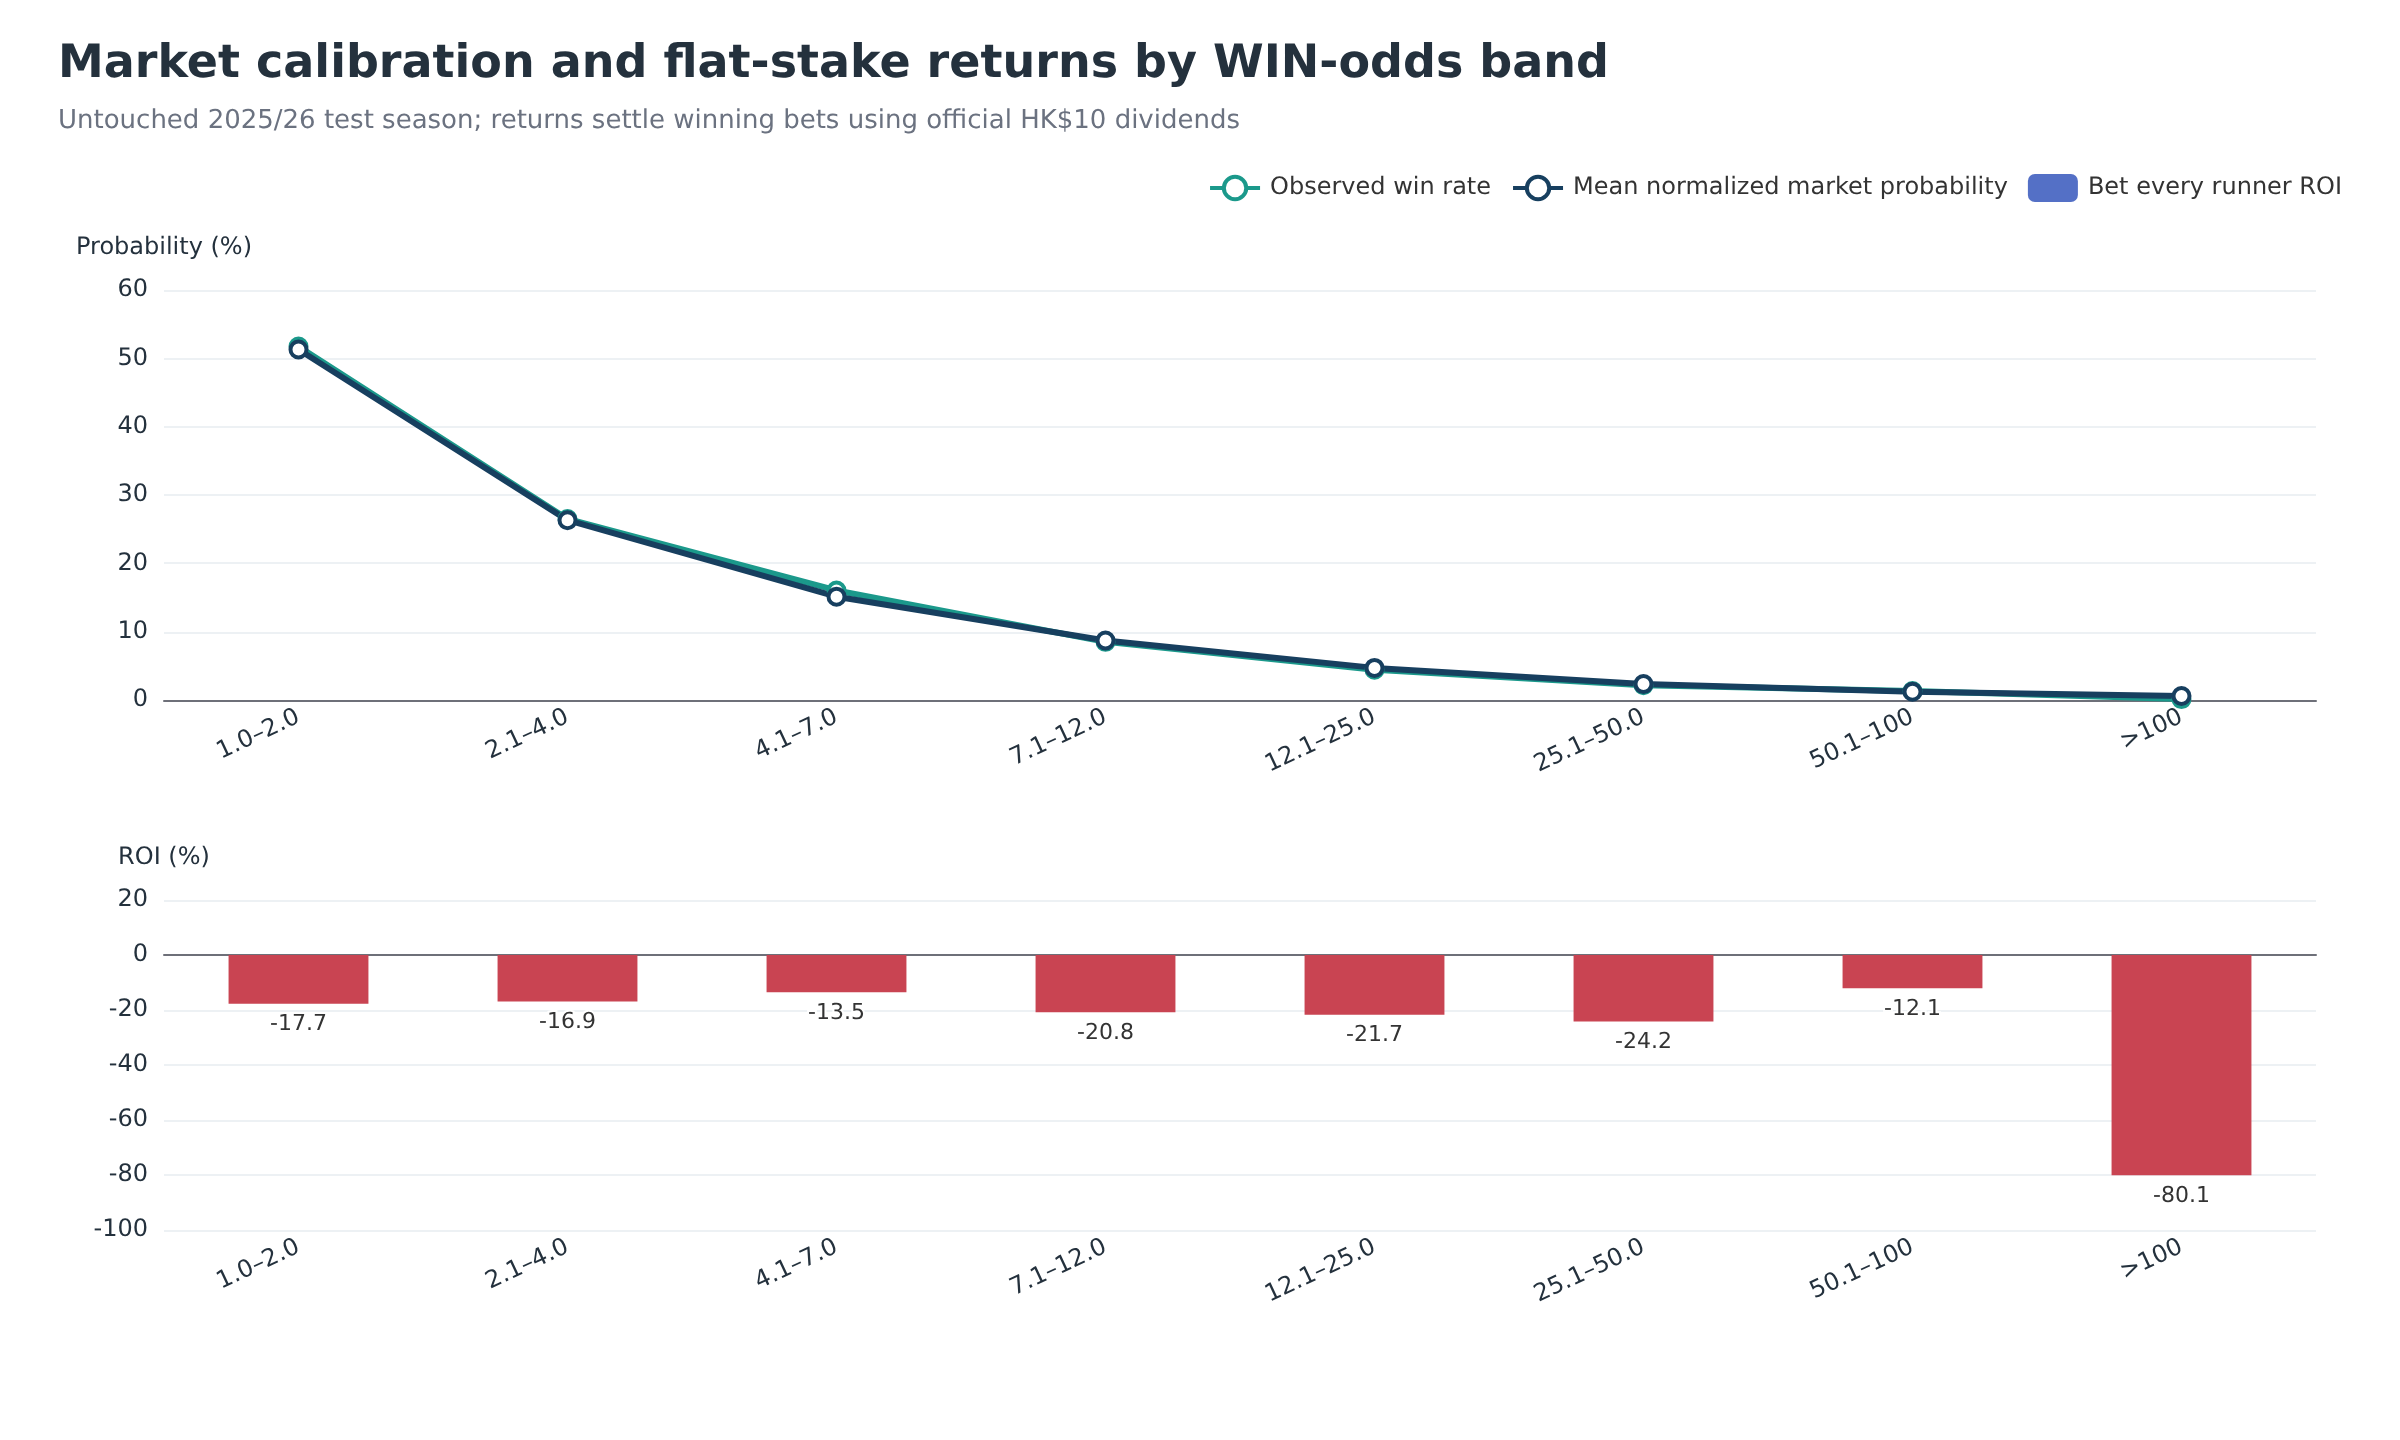
\includegraphics[width=0.98\textwidth]{odds_bands.png}
\caption{Test-season market calibration and unconditional flat-stake returns by displayed WIN-odds band. The upper panel uses all runners; the lower panel bets HK\$10 on every runner and settles from official dividends.}\label{fig:odds-bands}
\end{figure}

\subsection{Prespecified betting evaluation}\label{sec:results-betting}
The primary combined-logit value rule qualifies in 127 of 862 test races, spread across 68 meetings. It stakes HK\$1,270 and returns a net profit of HK\$91, corresponding to ROI 7.17\%. The strike rate is 14.17\%, mean displayed odds are 9.51, and maximum drawdown is HK\$287. Although the point estimate is positive, the meeting-cluster 95\% ROI interval is $[-49.56\%,77.19\%]$. Only 18 of the 127 selections win, so a small number of payouts materially affects the result. The appropriate conclusion is that the interim data are compatible with both meaningful gains and substantial losses, not that a profitable system has been demonstrated.

Alternative strategies are generally negative. Betting the primary model's top-probability runner in every race produces 29.35\% winners but loses HK\$1,399 on HK\$8,620 staked (ROI $-16.23\%$). This is less negative than the favourite-every-race ROI of $-19.94\%$, but both lose money. Combined-LightGBM value betting loses 2.12\% over 481 bets; fundamental-logit and fundamental-LightGBM value rules lose 31.85\% and 14.32\%, respectively. Betting every runner loses HK\$25,342.50 on HK\$107,600 staked (ROI $-23.55\%$). The contrast between top-one accuracy and negative return directly supports the project's separation of probability quality and economic value.

\begin{table}[htbp]
\centering
\caption{Selected test-season betting outcomes at HK\$10 flat stakes}\label{tab:betting-main}
\scriptsize
\setlength{\tabcolsep}{2.5pt}
\begin{tabular}{L{3.1cm} R{1.0cm} R{1.5cm} R{1.9cm} R{1.35cm} R{1.2cm} R{1.25cm} L{3.0cm}}
\toprule
\textbf{Strategy} & \textbf{Bets} & \textbf{Stake HK\$} & \textbf{Profit HK\$} & \textbf{ROI} & \textbf{Strike rate} & \textbf{Max DD HK\$} & \textbf{95\% ROI interval} \\
\midrule
Combined logit value & 127 & \num{1270} & $+91.00$ & $+7.17\%$ & 14.17\% & 287.00 & $[-49.56\%,77.19\%]$ \\
Combined logit top pick & 862 & \num{8620} & $-\num{1399.00}$ & $-16.23\%$ & 29.35\% & \num{1525.00} & $[-25.95\%,-7.09\%]$ \\
Combined LightGBM value & 481 & \num{4810} & $-102.00$ & $-2.12\%$ & 12.89\% & 529.50 & $[-30.61\%,28.67\%]$ \\
Fundamental logit value & 833 & \num{8330} & $-\num{2653.00}$ & $-31.85\%$ & 5.52\% & \num{3035.50} & $[-53.27\%,-9.16\%]$ \\
Fundamental LightGBM value & 840 & \num{8400} & $-\num{1203.00}$ & $-14.32\%$ & 6.19\% & \num{2755.00} & $[-39.16\%,12.25\%]$ \\
Favourite every race & 862 & \num{8620} & $-\num{1718.50}$ & $-19.94\%$ & 28.65\% & \num{1718.50} & $[-29.51\%,-10.58\%]$ \\
Every runner & \num{10760} & \num{107600} & $-\num{25342.50}$ & $-23.55\%$ & 8.01\% & --- & --- \\
\bottomrule
\end{tabular}
\source{Official WIN dividends settle winners. Intervals use 3,000 meeting-cluster resamples. The every-runner baseline has no selection bootstrap or drawdown entry.}
\end{table}

Figure~\ref{fig:cumulative-profit} shows the time path behind the summary statistics. The primary value balance rises through some parts of the season but also experiences extended flat and declining intervals; its final HK\$91 profit is small relative to the path's fluctuations and to total stakes. The favourite strategy declines much more persistently and ends at HK\$-1,718.50. A cumulative graph is useful for identifying sequence and drawdown, but it does not add independent evidence beyond the same 862 races. It should therefore be read together with, rather than instead of, the clustered intervals and sensitivity analysis.

\begin{figure}[htbp]
\centering
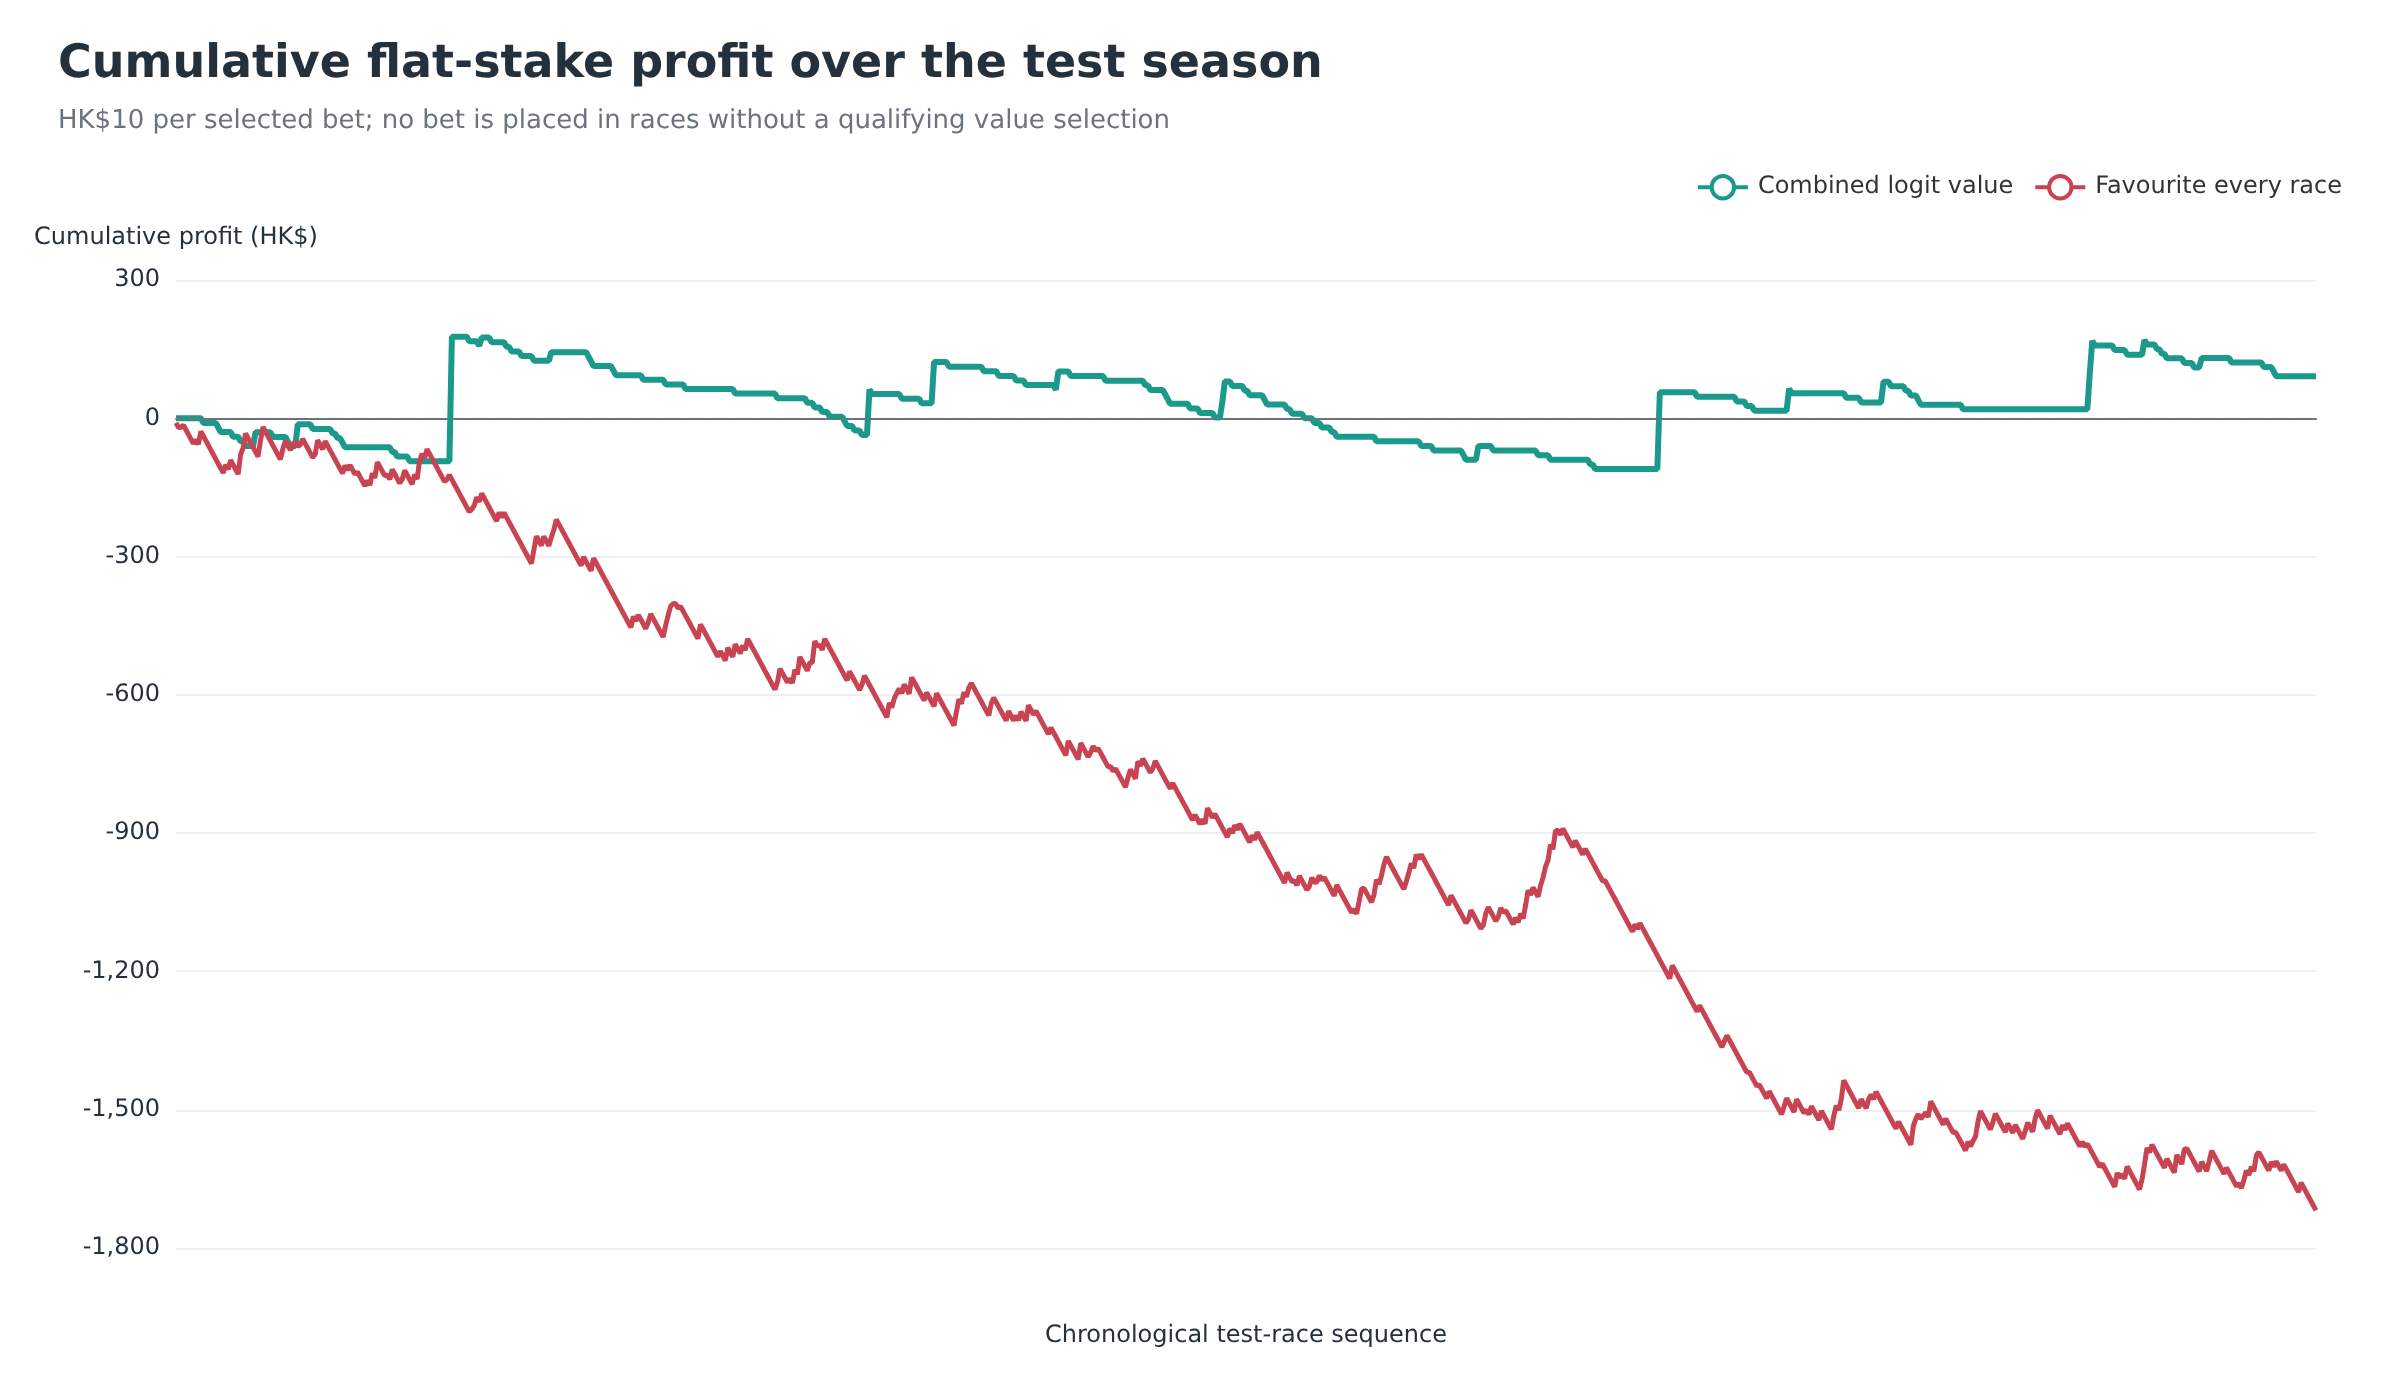
\includegraphics[width=0.97\textwidth]{cumulative_profit.png}
\caption{Cumulative test-season profit for the primary value rule and favourite-every-race baseline. Flat portions of the value series represent chronological races without a qualifying selection.}\label{fig:cumulative-profit}
\end{figure}

\subsection{Threshold sensitivity and robustness}\label{sec:results-sensitivity}
Figure~\ref{fig:sensitivity} varies the expected-value threshold and maximum odds for the primary model. The results are not monotone. With no edge requirement and an odds cap of 30, ROI is $-8.7\%$ over 269 bets; the prespecified 5\% edge and cap of 30 produce $+7.2\%$ over 127 bets; and a 10\% edge with the same cap produces $+65.9\%$ over only 48 bets. At a 20\% threshold, just four bets qualify and all lose, giving $-100\%$ ROI. No bets qualify at 30\%. Reducing the cap to ten under the 5\% rule produces $+5.5\%$ over 93 bets, whereas a cap of 20 produces $-1.1\%$ over 117.

These variations undermine any strong claim based on the positive primary cell. The most profitable cells contain fewer observations, and small changes in threshold move both the sign and magnitude of returns. The grid is therefore reported as an exploratory robustness diagnostic, not used to select a new ``optimal'' rule on the test season. A confirmatory final-stage analysis would need to freeze any revised rule using training/validation evidence and evaluate it on new data. At present, RQ4 is answered negatively in the robust sense: one positive point estimate exists, but profitability is not stable enough to support a reliable economic conclusion.

\begin{figure}[htbp]
\centering
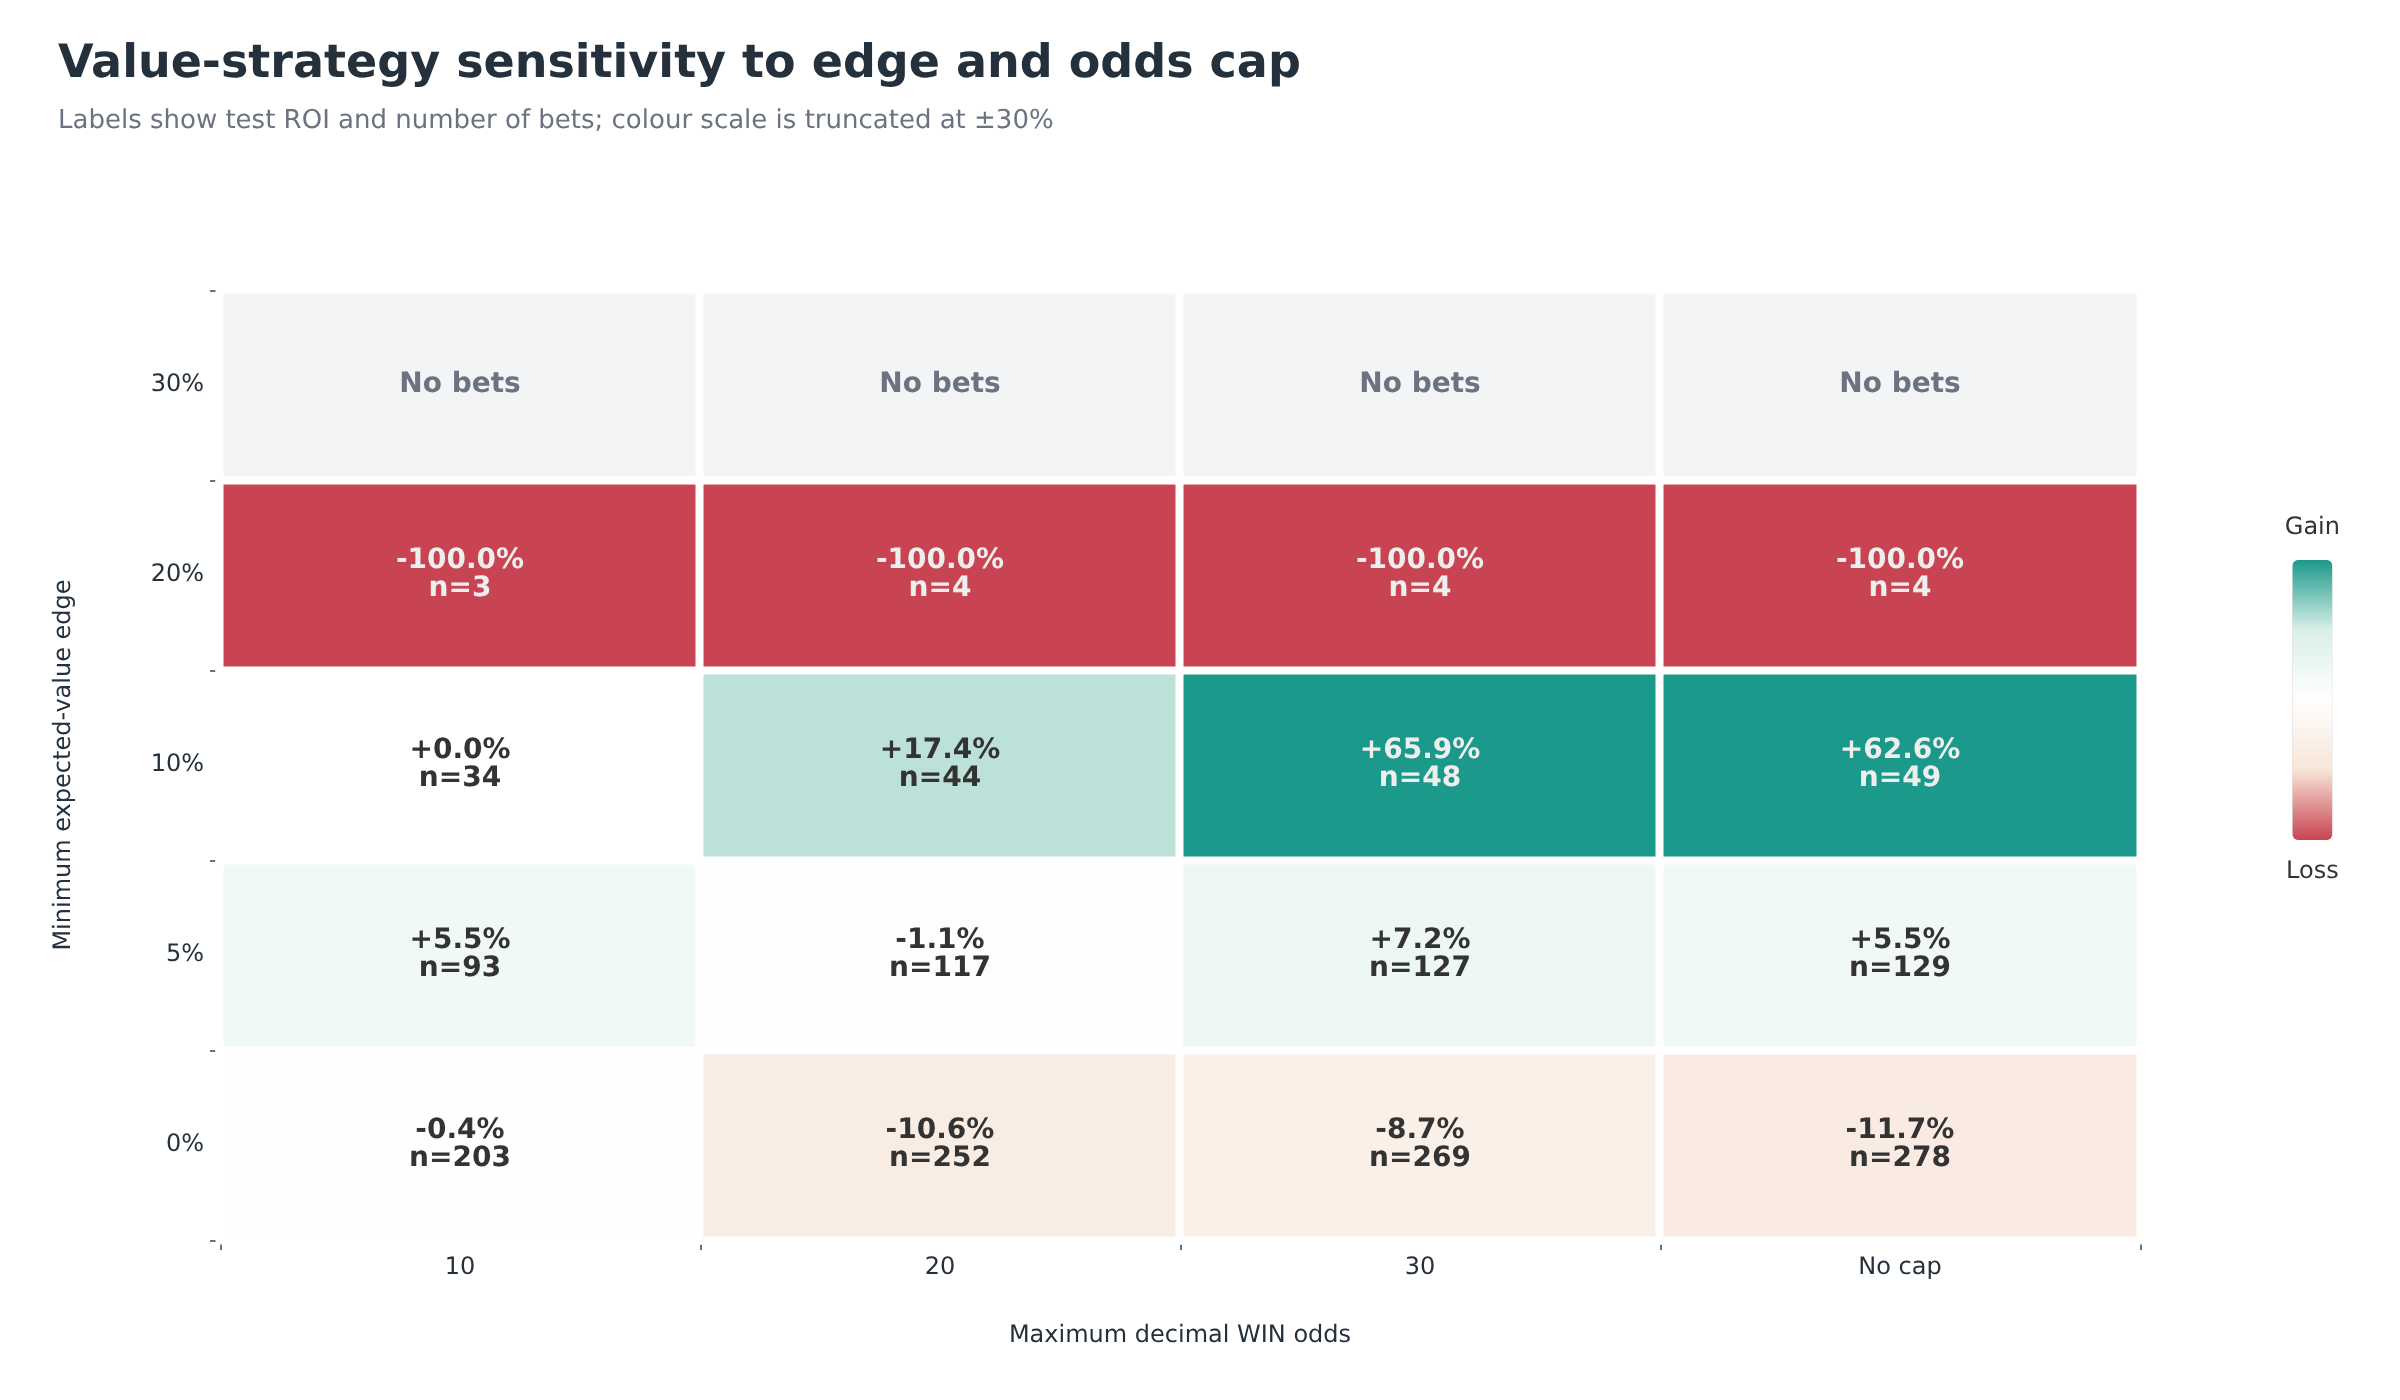
\includegraphics[width=0.97\textwidth]{betting_sensitivity.png}
\caption{Exploratory test-season sensitivity of the primary value rule. Labels show ROI and number of bets. The colour scale is truncated at $\pm30\%$ so that moderate cells remain distinguishable.}\label{fig:sensitivity}
\end{figure}

\section{Discussion and Validity Assessment}\label{sec:discussion}

\subsection{Interpretation of the research questions}\label{sec:discussion-rq}
For RQ1, the interim evidence supports a meaningful but limited fundamental signal. Both fundamental estimators outperform the uniform benchmark by a wide margin in log loss and top-one strike rate, yet their test log losses are approximately 0.214 above the market and their top-one rates are roughly five to six percentage points lower. The constructed histories therefore capture real information about relative performance, connections, and race conditions, but not enough to rival the information aggregated in final prices. This does not imply that fundamental variables have no value; it implies that their standalone forecasts should not be confused with the best available forecast when final market information is permitted.

For RQ2, race-normalized and temperature-adjusted probabilities are approximately calibrated at a global level, with small ECE values and reliability curves that broadly follow the diagonal. Nevertheless, local deviations remain and ECE has structural limitations, including the degenerate uniform-benchmark case. For RQ3, adding market information produces a dramatic improvement over fundamental models, but incremental improvement over the market itself is unresolved. The primary model's paired intervals for log loss, Brier loss, and top-one rate all include zero. The most defensible summary is therefore market-comparable performance in one test season, with no established incremental forecasting advantage.

For RQ4, the positive 7.17\% ROI for the primary value rule is interesting but evidentially weak. Its confidence interval is wide, it depends on 127 bets and 18 winners, and nearby thresholds produce materially different outcomes. The negative results for top-pick, favourite, every-runner, and fundamental value strategies show that most simple approaches lose after official settlement. Taken together, the findings do not establish either a universally efficient market or a usable inefficiency. They show that this particular model and dataset do not provide robust evidence of exploitable WIN value, while leaving open whether richer information and more realistic execution data could change the conclusion.

\subsection{Methodological lessons}\label{sec:discussion-lessons}
The first lesson is that problem representation matters. Treating runners as independent binary rows would obscure the fact that every race has a fixed choice set and would require an additional normalization step before proper evaluation. Conditional logit builds this constraint into estimation, while the LightGBM comparator receives it only at prediction time. Their similar fundamental test log losses suggest that the current feature set and sample do not produce a large advantage for either representation. This is a useful interim result because it directs future effort toward information and validation design rather than assuming that a more complex learner must improve performance.

The second lesson is that careful data auditing changes substantive results. Withdrawn horses initially appeared to make 383 races unusable; recognizing their HKJC status codes restored those races and corrected field sizes, overrounds, market probabilities, and histories. Likewise, official dividends matter because a rounded displayed price is not always identical to the actual payout. Finally, entity--race aggregation before shifting is necessary to prevent subtle same-race leakage for trainers and jockeys. These details are less visually appealing than model diagrams, but they protect the validity of every downstream metric.

The third lesson is that economic evaluation requires a different inferential mindset from prediction evaluation. The primary top-pick rule increases strike rate relative to favourites yet still loses money; the value rule earns a small profit despite lower predictive performance being statistically indistinguishable from the market; and the most profitable sensitivity cell is based on only 48 bets. Prediction metrics average over all races, whereas betting metrics condition on a model-selected, often long-priced subset. The final project should retain this separation and avoid using betting ROI as a substitute for probability scoring or vice versa.

\subsection{Threats to internal and statistical validity}\label{sec:discussion-limitations}
The most important threat is the use of final odds as predictors and decision prices. Final odds are available in the archived result page, but the dataset does not establish the exact moment at which a simulated bettor could observe them or submit a bet. In a pari-mutuel market, later wagers can move both the odds and dividend. The backtest therefore measures closing-price value, not guaranteed implementable profit. Obtaining timestamped odds near the off, specifying an information cutoff, and modeling slippage are necessary before making execution claims.

A second threat is sample and feature censoring. Histories begin in September 2021, so an established horse's first observed start in the dataset is not a true debut and early-season career features are left-censored. The current panel also lacks sectional times, speed figures, equipment changes, trackwork, veterinary information, detailed weather, and many other potentially informative variables. Non-finish codes are mapped to the worst finishing percentile, which is a transparent simplification but ignores differences among pulled-up, unseated, and disqualified outcomes. Dead heats are excluded, which has negligible sample-size impact but limits generality to the single-winner likelihood.

A third threat is residual selection and dependence. The validation season is used for penalties, temperatures, and primary-model selection, so repeated future experimentation on that season could gradually overfit it. The test sensitivity grid is explicitly exploratory, but reporting many cells still creates a risk that readers focus on the most favourable one. Meeting clustering addresses some shared shocks, yet it cannot model every source of dependence across nearby meetings or seasonal regimes. Percentile bootstrap intervals also do not include model-form, data-collection, or execution uncertainty.

\begin{table}[htbp]
\centering
\caption{Principal limitations, consequences, and planned mitigation}\label{tab:limitations}
\small
\begin{tabularx}{\textwidth}{L{3.2cm} Y Y}
\toprule
\textbf{Limitation} & \textbf{Why it matters} & \textbf{Planned response} \\
\midrule
Final-odds proxy & A closing-price backtest may not be executable at the displayed price. & Seek timestamped odds; impose an explicit cutoff; test slippage scenarios. \\
\addlinespace
Left-censored histories & Early observed horse and connection records omit pre-2021 experience. & Extend the lookback period and test warm-up exclusions or sensitivity to initial seasons. \\
\addlinespace
Incomplete handicapping information & Sectionals, equipment, trackwork, and other signals may be omitted. & Prioritize obtainable high-value features and document every additional source. \\
\addlinespace
Single test season & One season cannot establish temporal stability. & Add rolling-origin origins and reserve future data for confirmation. \\
\addlinespace
Validation reuse & Repeated tuning can overfit the validation year. & Keep a decision log and limit the remaining search to a small prespecified set. \\
\addlinespace
Exploratory threshold grid & Attractive cells can arise by chance or small samples. & Treat grid as diagnostic; validate any revised rule chronologically on new data. \\
\addlinespace
Simplified non-finish handling & Different non-completion mechanisms may carry different information. & Add indicator variables and compare alternative encodings. \\
\addlinespace
No market impact or rebate model & Real returns can differ for larger or eligible wagers. & Retain flat-stake baseline and add separately labeled execution scenarios. \\
\bottomrule
\end{tabularx}
\end{table}

\subsection{External validity and responsible interpretation}\label{sec:discussion-external}
The findings concern Hong Kong local WIN markets during 2021/22--2025/26. They should not be transported directly to bookmaker markets, other jurisdictions, place or exotic pools, or future seasons without revalidation. Different takeout rates, field sizes, racing programmes, information environments, and bettor behaviour can change both probability calibration and return distributions. Even within Hong Kong, performance may differ by course, surface, class, or distance. Subgroup analysis can reveal instability, but it must be interpreted with multiple-testing caution and adequate sample sizes.

There is also a responsible-communication requirement. A positive historical ROI is not a recommendation to bet, and the very wide interval in this study illustrates how limited the evidence is. The academic value of the project lies in transparent measurement, not in promoting gambling. The final report and presentation should preserve the research-use notice, display sample sizes next to returns, distinguish exploratory from prespecified findings, and avoid language such as ``guaranteed'', ``safe'', or ``proven profitable''. These practices improve both scientific and ethical quality.

\section{Remaining Work and Project Management}\label{sec:plan}

\subsection{Completed foundation and extension priorities}\label{sec:plan-priorities}
The interim stage has established the data, modeling, and evaluation infrastructure needed for the final stage. The immediate priority is no longer simply to collect more rows or test arbitrary algorithms. It is to address specific weaknesses identified by the empirical results: limited incremental information over the market, uncertain temporal stability, simplified treatment of non-finishers and early histories, and the gap between closing-price simulation and executable wagering. Extensions will therefore be evaluated against the current benchmarks with the same proper scores and official-dividend settlement, preserving comparability.

The modeling search will remain deliberately small. Priorities are a two-stage fundamental/market combination motivated by Benter, a compact ablation of recent-form and connection features, and one ranking-model extension if it can be validated without changing the WIN objective implicitly\cite{benter1994,harville1973}. Any new specification must first demonstrate validation improvement; test results will not be used to select among new variants. If these extensions fail to improve validation performance, the negative result will be retained and the simpler market and conditional-logit benchmarks will remain central.

\begin{table}[htbp]
\centering
\caption{Interim completion status and verifiable evidence}\label{tab:completion}
\small
\begin{tabularx}{\textwidth}{L{4.0cm} L{2.2cm} Y}
\toprule
\textbf{Work package} & \textbf{Status} & \textbf{Evidence produced} \\
\midrule
Official data collection & Complete & Five-season fixture/results panel, cached official pages, coverage table, source URLs, and zero request errors. \\
Cleaning and quality assurance & Complete & Withdrawal audit, dead-heat handling, complete-case checks, sample-flow table, and official-page spot checks. \\
Feature engineering & Complete for interim & Prior-only horse, distance, course, jockey, and trainer histories; race-relative and interaction variables. \\
Probability modeling & Complete for interim & Fundamental/combined conditional logit and LightGBM, validation penalty selection, and race-wise normalization. \\
Calibration and prediction evaluation & Complete for interim & Temperature scaling, metrics, reliability curves, feature importance, and paired predictive intervals. \\
Initial WIN backtest & Complete for interim & Official-dividend ledgers, ROI, drawdown, clustered ROI intervals, odds bands, and sensitivity grid. \\
Execution-realism analysis & Not complete & Requires timestamped odds or a defensible proxy and explicit slippage scenarios. \\
Final integration and presentation & In preparation & Final robustness analyses, report revision, supervisor feedback, and 8--10 minute slide narrative. \\
\bottomrule
\end{tabularx}
\end{table}

\subsection{Planned analytical extensions}\label{sec:plan-analysis}
The first extension is temporal robustness. Rolling-origin evaluation will train on expanding earlier windows and validate on successive later periods, recording score distributions rather than relying only on the single 2024/25 validation year. This analysis will assess whether the market temperature, conditional-logit penalty, and combined-model advantage are stable. It will also provide a more defensible basis for freezing a revised betting threshold. The existing 2025/26 test results will remain labeled as interim hold-out evidence; if they are used during model development, a genuinely new future period will be required for any subsequent confirmatory claim.

The second extension is information quality. A longer historical lookback would reduce left censoring, while separate non-finish indicators would replace some of the information lost by assigning one worst percentile. Course/distance-specific form and draw interactions will be examined through ablation rather than expanded indiscriminately. Where new official or otherwise verifiable fields can be obtained consistently, sectional timing and equipment information are higher priorities than additional transformations of final odds. Each feature family will be assessed by validation log loss, calibration, stability, and interpretability.

The third extension is decision realism. The current flat-stake analysis will remain the transparent baseline. Scenario analysis may vary the price available at execution, apply conservative slippage, and quantify how often a qualifying signal disappears. Kelly or fractional-Kelly staking will be considered only as a secondary mathematical comparison because it magnifies probability-estimation error and drawdown risk. No staking system will be presented as converting a negative or unresolved edge into a reliable profit. Rebate and market-impact scenarios, if included, will be separately labeled assumptions rather than mixed into the official-dividend baseline.

\subsection{Timeline and deliverables}\label{sec:plan-timeline}
Table~\ref{tab:timeline} schedules the remaining work around the interim deadline of 26 November 2026. The dates are project-management targets rather than assumed university deadlines beyond those supplied for the interim report. Supervisor feedback is an explicit gate before major model expansion, because it can help distinguish necessary methodological work from low-value complexity. Final submission and presentation dates marked TBC will be aligned with official course instructions when available.

Versioned checkpoints will contain the report source, analysis scripts, manifests, and result tables at each milestone. This reduces the risk that a late code change silently alters earlier numbers. Before final submission, a clean rerun will compare regenerated metrics with the reported tables, every figure will be checked against its source file, and all references and cross-references will be compiled and visually inspected. Time is reserved for Turnitin processing, supervisor review, the separate declaration form, and contingency rather than treating them as last-minute administrative tasks.

\begin{table}[htbp]
\centering
\caption{Remaining-project timeline}\label{tab:timeline}
\small
\begin{tabularx}{\textwidth}{L{3.2cm} Y L{4.1cm}}
\toprule
\textbf{Target period} & \textbf{Planned work} & \textbf{Checkpoint / output} \\
\midrule
By 26 Nov 2026, 15:00 & Complete supervisor review, finalize interim PDF/Word submission, upload through the FYP system, and allow Turnitin generation time. & Interim report and separate signed declaration form. \\
\addlinespace
27 Nov--15 Dec 2026 & Consolidate feedback; freeze extension priorities; implement longer-history and non-finish sensitivity checks. & Revised data-quality and feature-ablation note. \\
\addlinespace
16 Dec 2026--31 Jan 2027 & Run rolling-origin comparisons and a small prespecified two-stage/model-ablation study. & Validated model-comparison table and frozen final methodology. \\
\addlinespace
February 2027 & Investigate timestamped price availability; conduct execution and slippage scenarios; complete robustness analysis. & Betting-validity chapter and final result artifacts. \\
\addlinespace
March 2027 & Integrate final report, repeat clean reproduction checks, and obtain supervisor feedback. & Near-final written report. \\
\addlinespace
April 2027 or official deadline & Revise, proofread, compile, and submit final materials; archive reproducible package. & Final report and reproducibility archive. \\
\addlinespace
Presentation window (TBC) & Rehearse an 8--10 minute presentation and prepare Q\&A evidence slides. & Slide deck, timing rehearsal, and backup results. \\
\bottomrule
\end{tabularx}
\end{table}

\subsection{Presentation and Q\&A preparation}\label{sec:plan-presentation}
The presentation will tell one coherent empirical story rather than reciting every feature. A nine-minute target leaves margin within the required 8--10 minutes. The proposed allocation is 45 seconds for the problem and research questions, 60 seconds for official data and chronological splitting, 105 seconds for race probability and leakage-safe methods, 120 seconds for prediction and calibration findings, 105 seconds for betting and uncertainty, 60 seconds for limitations, and 45 seconds for remaining work and the conclusion. The central visual sequence will be the sample split, model log-loss comparison, reliability plot, and betting ROI/sensitivity summary.

Backup slides will contain the full metric table, feature definitions, betting ledger summary, paired intervals, and threshold grid so that questions can be answered without overcrowding the main narrative. Likely Q\&A topics include why independent binary classification is insufficient, how trainer leakage is prevented, why final odds limit execution claims, why accuracy does not imply profit, and whether the positive value ROI proves an edge. Rehearsal will use a timer and require concise answers that refer to actual tables or equations. If a question concerns unavailable evidence, the response will identify the limitation and planned test rather than speculate.

\section{Conclusion}\label{sec:conclusion}
This interim report has converted a broad interest in horse-racing analytics into a reproducible mathematical and empirical study of race probability and WIN-betting decisions. The completed pipeline collects official HKJC data, audits withdrawn and dead-heat records, constructs prior-only historical features, fits conditional-logit and LightGBM models under fundamental and combined information sets, calibrates on a later validation season, and evaluates on an untouched 2025/26 test season. The resulting sample of \num{4207} races and \num{51068} starters is large enough to reveal a clear hierarchy: historical features are informative, final market probabilities are substantially stronger, and the current combined models offer no resolved improvement over that market benchmark.

The betting analysis reinforces the importance of evaluating decisions separately from predictions. The primary combined-logit value rule earns HK\$91 on HK\$1,270 staked, but its 7.17\% ROI has a 95\% meeting-cluster interval of $[-49.56\%,77.19\%]$ and is unstable across nearby thresholds. Top-pick, favourite, every-runner, and fundamental value strategies lose money under official-dividend settlement. These results are not evidence that profitable betting is impossible, and they are not proof of perfect market efficiency. They demonstrate that the present interim evidence does not justify a robust profitability claim and that small positive samples must be communicated with their uncertainty.

Semester 2 will therefore prioritize temporal robustness, market-anchored model upgrades, information quality, and execution realism over unrestricted model searching. Rolling-origin evaluation, a small shrinkage and ablation programme, improved historical coverage, and timestamped price scenarios offer direct tests of the current limitations. The existing scripts, tables, figures, and source-linked runner panel provide a stable foundation for that work. By preserving chronological discipline, official settlement, and transparent reporting, the full-year capstone can produce a defensible final contribution regardless of whether a genuine economic edge is ultimately found.


\clearpage
\begingroup
\small
\setstretch{0.96}
\setlength{\parskip}{0.25em}
\bibliography{references}
\endgroup

\clearpage
\appendix
\section{Additional Numerical Results}\label{app:numerical}

\subsection{Complete betting summary}\label{app:betting}
Table~\ref{tab:betting-full} preserves the full strategy comparison, including top-pick results omitted from the main betting table for readability. The intervals reveal different types of evidence. Some negative strategies have intervals entirely below zero, whereas the primary value rule and several other value variants have intervals spanning both gains and losses. The combined-LightGBM value strategy is close to break-even in its point estimate but negative; the fundamental-LightGBM value point estimate is more negative while its interval still crosses zero. These differences show why ranking strategies by point ROI alone would be misleading.

Top-pick strategies place exactly one bet in every test race, whereas value strategies have variable coverage. Stake totals therefore differ, and ROI rather than raw profit is the appropriate scale-free comparison. Nevertheless, ROI does not convey path risk by itself, so maximum drawdown is included. All values can be reconstructed from the bet-level files listed in Appendix~\ref{app:reproduction}.

\begin{table}[htbp]
\centering
\caption{Complete test-season betting summary}\label{tab:betting-full}
\scriptsize
\setlength{\tabcolsep}{3.2pt}
\begin{tabular}{L{4.2cm} R{1.0cm} R{1.5cm} R{1.4cm} R{1.5cm} R{1.6cm} L{3.0cm}}
\toprule
\textbf{Strategy} & \textbf{Bets} & \textbf{Stake HK\$} & \textbf{ROI} & \textbf{Strike rate} & \textbf{Max DD HK\$} & \textbf{95\% ROI interval} \\
\midrule
Fundamental logit value & 833 & \num{8330} & $-31.85\%$ & 5.52\% & \num{3035.50} & $[-53.27\%,-9.16\%]$ \\
Fundamental logit top pick & 862 & \num{8620} & $-24.40\%$ & 22.85\% & \num{2171.00} & $[-34.89\%,-13.76\%]$ \\
Fundamental LightGBM value & 840 & \num{8400} & $-14.32\%$ & 6.19\% & \num{2755.00} & $[-39.16\%,12.25\%]$ \\
Fundamental LightGBM top pick & 862 & \num{8620} & $-16.14\%$ & 23.43\% & \num{1763.50} & $[-27.85\%,-3.90\%]$ \\
Combined logit value & 127 & \num{1270} & $+7.17\%$ & 14.17\% & 287.00 & $[-49.56\%,77.19\%]$ \\
Combined logit top pick & 862 & \num{8620} & $-16.23\%$ & 29.35\% & \num{1525.00} & $[-25.95\%,-7.09\%]$ \\
Combined LightGBM value & 481 & \num{4810} & $-2.12\%$ & 12.89\% & 529.50 & $[-30.61\%,28.67\%]$ \\
Combined LightGBM top pick & 862 & \num{8620} & $-17.20\%$ & 28.54\% & \num{1760.00} & $[-27.23\%,-7.13\%]$ \\
Favourite every race & 862 & \num{8620} & $-19.94\%$ & 28.65\% & \num{1718.50} & $[-29.51\%,-10.58\%]$ \\
Every runner & \num{10760} & \num{107600} & $-23.55\%$ & 8.01\% & --- & --- \\
\bottomrule
\end{tabular}
\end{table}

\subsection{Complete paired predictive comparisons}\label{app:predictive-intervals}
The paired comparisons in Table~\ref{tab:predictive-full} use the market as the reference within each meeting resample. Negative log-loss and Brier differences favour the candidate; positive top-one differences favour the candidate. Fundamental models are clearly worse than the market on all three measures. Combined logit has intervals crossing zero throughout. Combined LightGBM has a positive log-loss interval, indicating worse performance than the market, while its Brier and top-one intervals still include zero.

These intervals supplement rather than replace the metric table. A difference can be small in practical terms even when an interval excludes zero, and an interval crossing zero does not prove exact equivalence. The purpose is to prevent overinterpretation of tiny numerical differences and to show the scale of unresolved temporal and meeting-level variation.

\begin{table}[htbp]
\centering
\caption{Paired test differences against the calibrated market benchmark}\label{tab:predictive-full}
\small
\begin{tabular}{L{4.1cm} L{2.5cm} R{2.3cm} R{4.3cm}}
\toprule
\textbf{Candidate} & \textbf{Metric} & \textbf{Difference} & \textbf{95\% interval} \\
\midrule
Fundamental logit & Log loss & $+0.214983$ & $[+0.170234,+0.260564]$ \\
Fundamental logit & Brier loss & $+0.050562$ & $[+0.037306,+0.063952]$ \\
Fundamental logit & Top-one rate & $-5.800$ pp & $[-9.122,-2.532]$ pp \\
\addlinespace
Fundamental LightGBM & Log loss & $+0.214035$ & $[+0.167856,+0.260613]$ \\
Fundamental LightGBM & Brier loss & $+0.050418$ & $[+0.036758,+0.064291]$ \\
Fundamental LightGBM & Top-one rate & $-5.220$ pp & $[-8.305,-2.191]$ pp \\
\addlinespace
Combined logit & Log loss & $-0.000328$ & $[-0.008867,+0.008288]$ \\
Combined logit & Brier loss & $+0.000650$ & $[-0.002300,+0.003498]$ \\
Combined logit & Top-one rate & $+0.696$ pp & $[-0.692,+2.100]$ pp \\
\addlinespace
Combined LightGBM & Log loss & $+0.014841$ & $[+0.000977,+0.029003]$ \\
Combined LightGBM & Brier loss & $+0.003315$ & $[-0.000887,+0.007564]$ \\
Combined LightGBM & Top-one rate & $-0.116$ pp & $[-2.191,+2.050]$ pp \\
\bottomrule
\end{tabular}
\end{table}

\section{Reproducibility Guide}\label{app:reproduction}
The source package separates collection, analysis, visualization, and reporting. The \texttt{data/} directory contains fixture, raw race, raw runner, coverage, manifest, and engineered-panel files; \texttt{results/} contains every table used in the report; and \texttt{figures/} contains the rendered ECharts images. The \texttt{report/} directory contains the split \LaTeX{} files and bibliography. Original compressed HTML pages are retained in the working archive but are not required to rerun the analysis from the included raw CSV files.

The principal reproduction commands are shown below. Collection requires network access and should be run only when refreshing the source data. Analysis and figure generation can run from the included data files. Compiling from \texttt{report/} preserves the relative path to \texttt{figures/}. Package versions and operating-system details should be recorded in the final archive before submission.

\begin{verbatim}
# Optional: refresh official data (network required)
python3 scripts/collect_hkjc.py --workers 16

# Rebuild features, models, metrics, predictions, and betting outputs
python3 scripts/analyze.py

# Render static ECharts figures
python3 scripts/make_figures.py

# Compile the report from the report directory
cd report
tectonic -X compile main.tex
\end{verbatim}

\begin{table}[htbp]
\centering
\caption{Key reproducibility artifacts}\label{tab:artifacts}
\small
\begin{tabularx}{\textwidth}{L{5.6cm} Y}
\toprule
\textbf{Path} & \textbf{Contents} \\
\midrule
\path{data/collection_manifest.json} & Retrieval time, seasons, meeting/race/runner totals, candidate pages, and request errors. \\
\path{data/coverage.csv} & Scheduled and collected race counts for every fixture meeting. \\
\path{data/runners_raw.csv} & Source-linked runner records, final odds, and official winner dividends. \\
\path{data/model_runners.csv} & Clean starter panel with chronological features for every included runner. \\
\path{results/model_metrics.csv} & Validation/test scores and fitted temperatures. \\
\path{results/test_predictions.csv} & Runner-level probabilities for every model on the untouched test season. \\
\path{results/predictive_comparison_intervals.csv} & Paired meeting-bootstrap differences against market. \\
\path{results/betting_summary.csv} & Stakes, profits, ROI, strike rate, drawdown, and clustered ROI intervals. \\
\path{results/bets_*.csv} & Auditable selection-level betting ledgers. \\
\path{results/betting_sensitivity.csv} & Complete edge/odds-cap grid with sample sizes. \\
\path{results/feature_importance.json} & LightGBM gain values and conditional-logit coefficients. \\
\bottomrule
\end{tabularx}
\end{table}

\section{Administrative Submission Checklist}\label{app:admin}
The following checklist comes from the interim-report instructions supplied for this capstone. It is included for project management and does not replace official course guidance. All placeholders on the title page must be completed and the output file renamed before submission. The supervisor should review the actual final upload candidate, not merely an earlier draft.

\begin{tcolorbox}[capstonebox]
\begin{enumerate}
    \item Replace \placeholder{STUDENT NAME}, \placeholder{STUDENT ID}, \placeholder{SUPERVISOR NAME}, department, and institution placeholders.
    \item Obtain supervisor review and incorporate agreed corrections before submission.
    \item Rename the file using \path{(Your Name) (Student ID)_Capstone Interim report.xxx}, consistent with the supplied example \path{ChanTaiMan12345678D_Capstone Interim report.pdf}.
    \item Submit the PDF or Word document through the Final Year Project System by \textbf{26 November 2026 at 15:00}.
    \item Upload through Blackboard for Turnitin and allow sufficient report-generation time. The stated acceptable similarity is \textbf{30\%}.
    \item Submit the separate Capstone Project Interim Report Declaration Form signed by the student and supervisor(s), as required.
    \item Retain the source package, result manifests, and submitted PDF for audit and final-project continuity.
    \item Prepare for the eventual \textbf{8--10 minute presentation followed by Q\&A}; rehearse timing and maintain backup evidence slides.
\end{enumerate}
\end{tcolorbox}

\begin{tcolorbox}[cautionbox]
\textbf{Before using this document as the official submission.} The student must verify the current course instructions, provide identity details, complete institutional declarations, and obtain supervisor approval. The analytical content is complete for the interim stage, but no institutional template or grading rubric was supplied for this draft.
\end{tcolorbox}


\end{document}
